\section{CPEs and Research Data}
\label{section:cpe_research_data}

This chapter lists all \glspl{cpe} being analyzed, including the manufacturer name, the model number, and the transmission medium supported by the device. Each device is assigned an identifier that is used throughout this work.

Then it is explained how each \gls{cpe} is prepared before any data is collected or any experiment is executed. The state that the \gls{cpe} is put in resembles its state as soon as the equipment is installed by the \gls{isp} on the customer’s home.

Finally some data is collected from the device enclosure, the wireless network being broadcasted, the management interfaces, and the configuration file of each \gls{cpe}. This data is analyzed in the next chapters.

\subsection{Subjects}

The chosen \gls{isp} has two main offerings for their residential Internet service, copper and fiber. For each transmission medium, the \gls{isp} deploys different equipment as a residential gateway, that have been majorly manufactured by Askey and MitraStar in recent years.

This study will analyze 8 of those \gls{cpe}s, as specified on Table \ref{table:cpes_identifiers}. An equal number of copper and fiber devices was selected, as well as the number of Askey and MitraStar equipment.

\begin{table}[h]
    \makebox[\linewidth]{
        \begin{tabular}{c|c|c|c}
            \thead{\gls{cpe} Identifier} & \thead{Transmission Medium} & \thead{Manufacturer Name} & \thead{Model Number} \\
            \hline
            \gls{cpe}-0 & Copper & Askey & \texttt{RTA9227W-D112} \\
            \gls{cpe}-1 & Copper & Askey & \texttt{RTV9015VW} \\
            \gls{cpe}-2 & Copper & MitraStar & \texttt{DSL-100HN-T1-NV} \\
            \gls{cpe}-3 & Copper & MitraStar & \texttt{DSL-2401HN2-E1C} \\
            \gls{cpe}-4 & Fiber & Askey & \texttt{RTF3505VW-N2} \\
            \gls{cpe}-5 & Fiber & Askey & \texttt{RTF8115VW} \\
            \gls{cpe}-6 & Fiber & MitraStar & \texttt{GPT-2541GNAC-N1} \\
            \gls{cpe}-7 & Fiber & MitraStar & \texttt{GPT-2731GN2A4P} \\
        \end{tabular}
    }
    \caption{Identifiers of the \gls{cpe}s}
    \label{table:cpes_identifiers}
\end{table}

The \glspl{cpe} analyzed include all models that were leased by the \gls{isp} to the customers part of the research. Other models were incorporated into the analysis based on a list of devices on the \gls{isp} support page \cite{vivo_configuraraparelhos}.

\FloatBarrier

\subsection{Preparation}

Before any test was performed, each device had its latest \gls{isp}-provided firmware installed and was factory reset. Throughout the research, this is considered the baseline state of each device and represents a \gls{cpe} that had no intervention since the \gls{isp} had it installed on the customer’s home.

The firmware for each device was acquired by sending \gls{cwmp} Inform requests to the \gls{isp} \gls{acs} on behalf of the \gls{cpe} with the script of Appendix \ref{appendix:cwmp_dev_emu}. If the firmware was outdated, then a \gls{cwmp} Download Firmware Upgrade Image request would be received as the response, as shown in Figure \ref{figure:cwmp_download_firmware_upgrade_image}.

\begin{figure}[h]
    \centering
    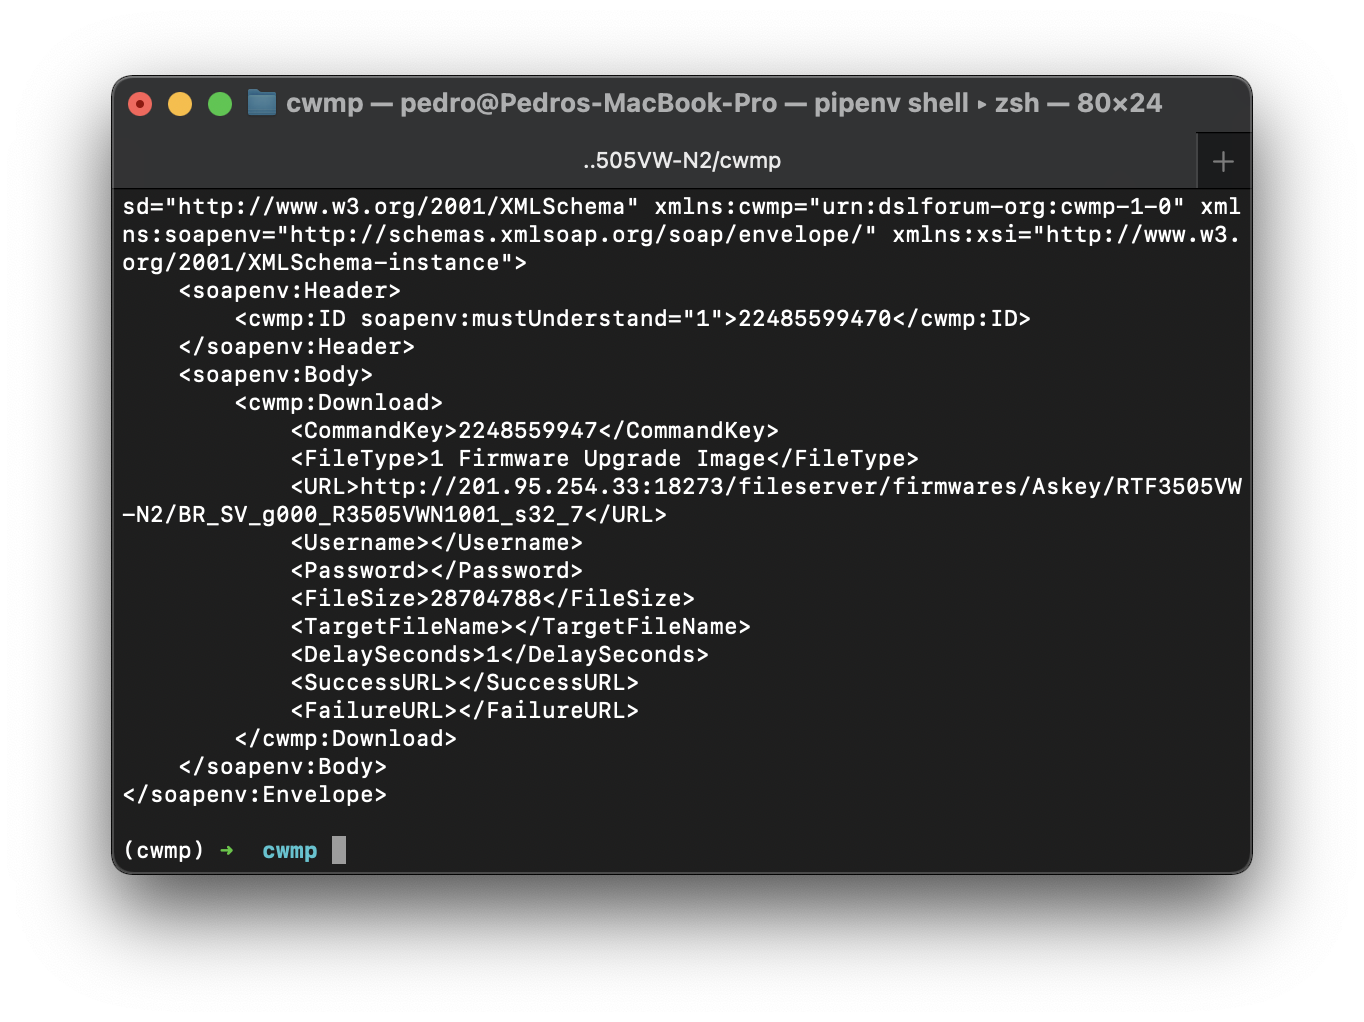
\includegraphics[width=\linewidth]{contents/cpes-and-research-data/preparation/cwmp-download-firmware-upgrade-image.png}
    \caption{\gls{cwmp} Download Firmware Upgrade Image}
    \label{figure:cwmp_download_firmware_upgrade_image}
\end{figure}

\gls{cpe}-0 and \gls{cpe}-1 never received firmware upgrade requests from \gls{acs}, no matter what version was set on the \gls{cwmp} Inform request. Looking into the firmware repository of the \gls{isp}, it was found that newer firmware was indeed available for download. But after further inspection, it was verified that both \glspl{cpe} are not able to have their firmware upgraded.

The experiments on \gls{cpe}-0 and \gls{cpe}-1 proceeded with the outdated firmware. All other devices were upgraded via the \gls{http} management interface with their respective firmware images, as shown on the Table \ref{table:cpes_firmwares}. Then, all \glspl{cpe} were factory reset by holding the reset button, located on the rear of each device, for 10 second.

\begin{table}[h]
    \makebox[\linewidth]{
        \begin{tabular}{c|c}
            \thead{\gls{cpe} Identifier} & \thead{Firmware Version} \\
            \hline
            \gls{cpe}-0 & \texttt{BR\_SO\_RTK\_V5.1.8j} \\
            \gls{cpe}-1 & \texttt{BR\_SO\_RTK\_V6.1.8t} \\
            \gls{cpe}-2 & \texttt{BR\_SA\_113WUK0b8} \\
            \gls{cpe}-3 & \texttt{BR\_SA\_g003\_114WUQ0b18} \\
            \gls{cpe}-4 & \texttt{BR\_SV\_g000\_R3505VWN1001\_s32\_7} \\
            \gls{cpe}-5 & \texttt{BR\_SG\_g11.11\_RTF\_TEF001\_V6.54\_V014} \\
            \gls{cpe}-6 & \texttt{BR\_SV\_1.00(VNZ.0)b18} \\
            \gls{cpe}-7 & \texttt{BR\_SV\_1.11(WVK.0)b18} \\
        \end{tabular}
    }
    \caption{Firmwares of the \gls{cpe}s}
    \label{table:cpes_firmwares}
\end{table}

With the devices set to their baseline, a computer was connected to one of \gls{cpe}’s \gls{lan} ports via an Ethernet cable and was able to acquire an \gls{ip} address from the \gls{dhcp} server running on the \gls{cpe}, as shown in Figure \ref{figure:wired_connection_to_the_cpe}. The gateway and \gls{dns} servers were set to the \gls{cpe}’s \gls{ip} address, \url{192.168.15.1} for all \glspl{cpe} in the research.

\begin{figure}[h]
    \centering
    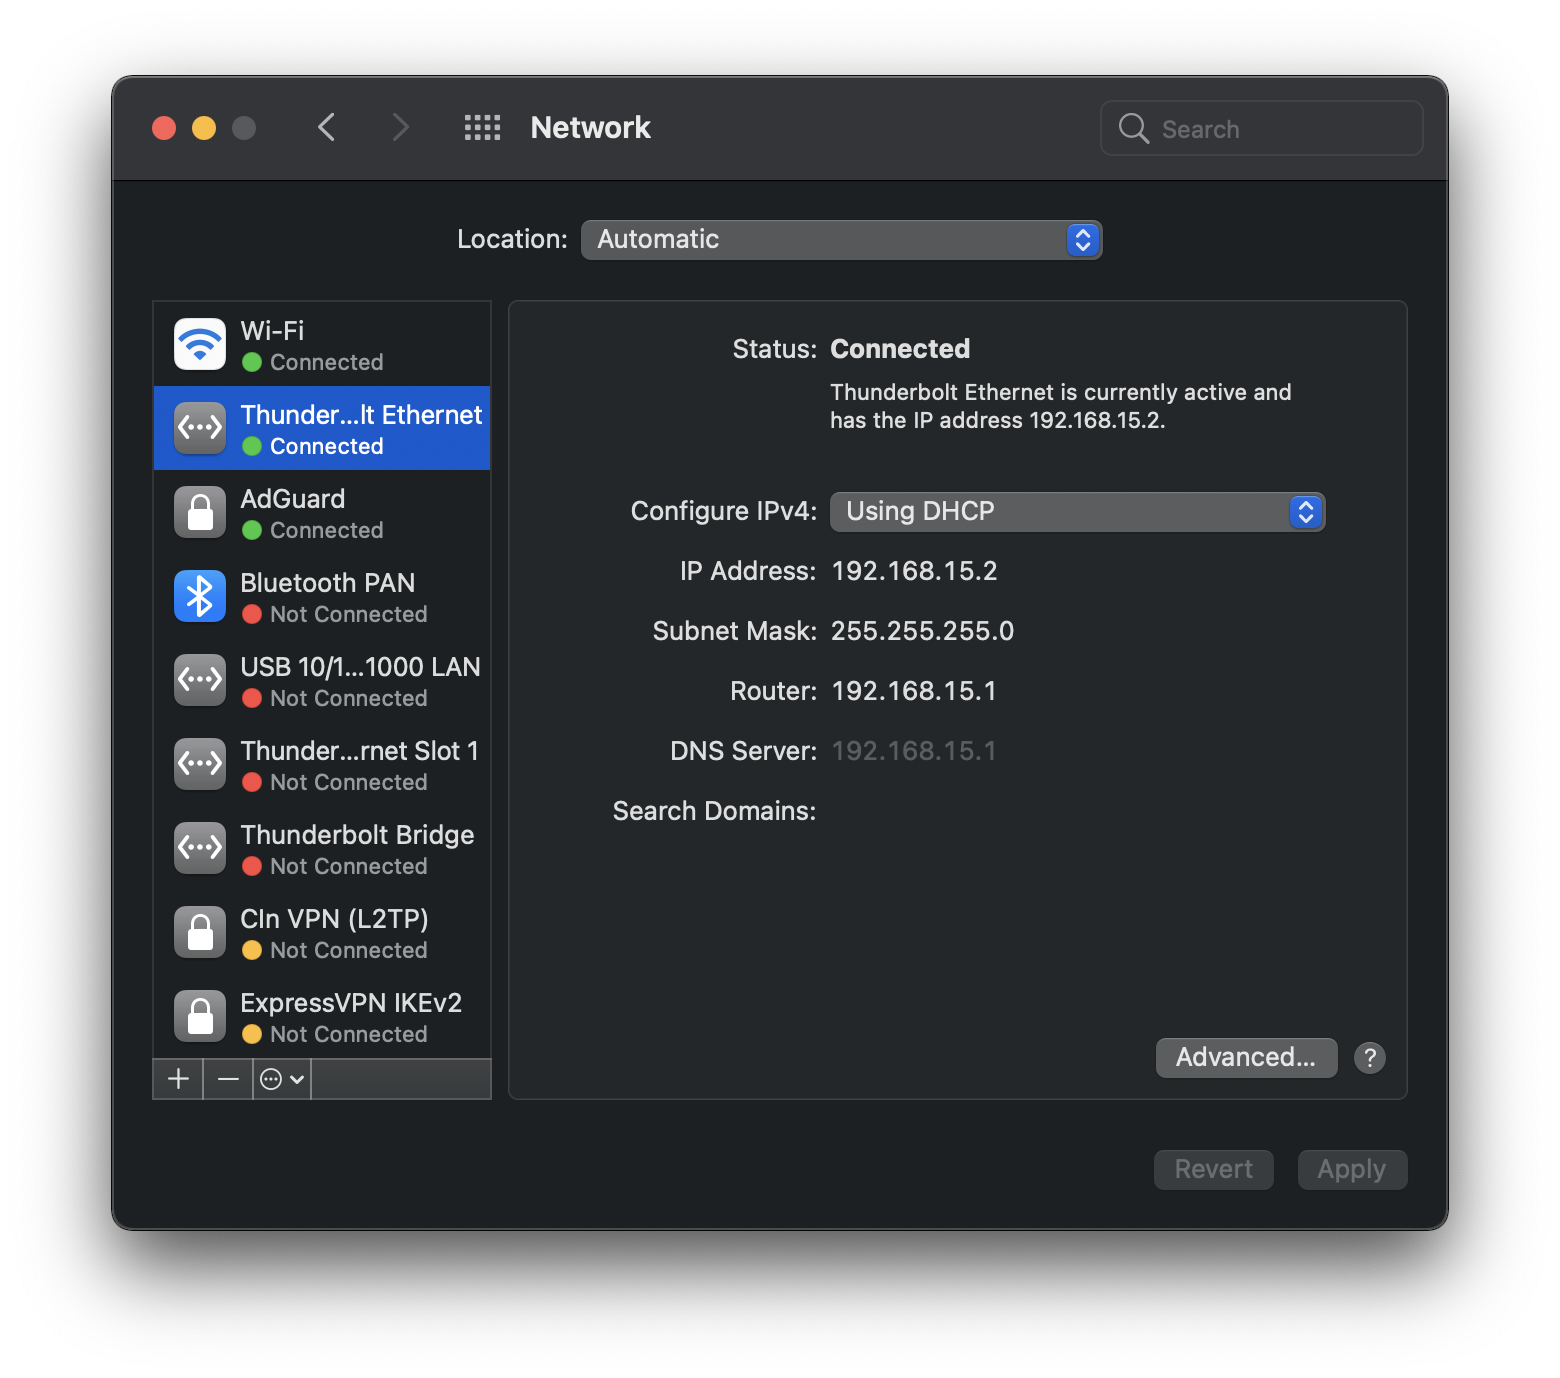
\includegraphics[width=\linewidth]{contents/cpes-and-research-data/preparation/wired-connection-to-the-cpe.png}
    \caption{Wired Connection to the \gls{cpe}}
    \label{figure:wired_connection_to_the_cpe}
\end{figure}

\FloatBarrier

\subsection{Operating System}

Most of the \glspl{cpe} run on the 32-bit \gls{mips} version of the Linux Kernel. The identification process was made by either executing commands on the device’s shell, as shown in Figure \ref{figure:checking_cpe_operating_system}, or by inspecting the firmware image installed. Unfortunately, not all devices had their operating system identified, they most likely don’t run Linux. 

\begin{figure}[h]
    \centering
    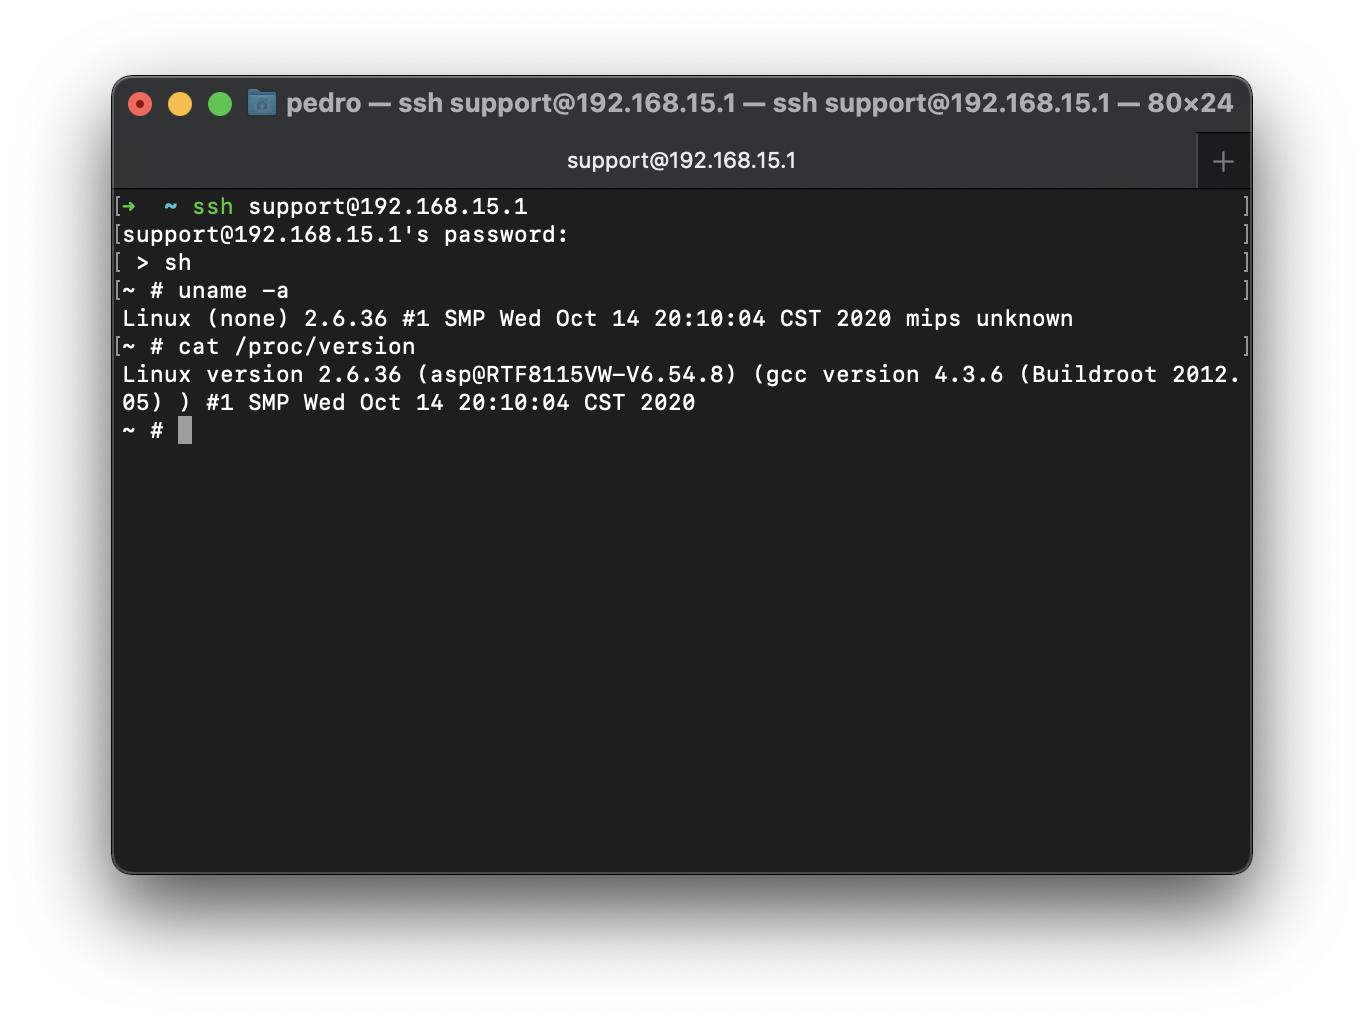
\includegraphics[width=\linewidth]{contents/cpes-and-research-data/operating-system/checking-cpe-operating-system.png}
    \caption{Checking \gls{cpe} Operating System}
    \label{figure:checking_cpe_operating_system}
\end{figure}

Table \ref{table:cpes_oses} presents the operating system identified on each \gls{cpe}.

\begin{table}[h]
    \makebox[\linewidth]{
        \begin{tabular}{c|>{\centering\arraybackslash}m{\linewidth}}
            \thead{\gls{cpe} Identifier} & \thead{Operating System} \\
            \hline
            \gls{cpe}-0 & unknown \\
            \gls{cpe}-1 & unknown \\
            \gls{cpe}-2 & unknown \\
            \gls{cpe}-3 & unknown \\
            \gls{cpe}-4 & \texttt{Linux version 3.4.11-rt19+ (openwrt@sw3-pc) (gcc version 4.6.2 (Buildroot 2011.11) ) \#1 SMP PREEMPT Thu Jun 18 13:46:11 CST 2020} \\
            \gls{cpe}-5 & \texttt{Linux version 2.6.36 (asp@RTF8115VW-V6.54.8) (gcc version 4.3.6 (Buildroot 2012.05) ) \#1 SMP Wed Oct 14 20:10:04 CST 2020} \\
            \gls{cpe}-6 & \texttt{Linux version 3.4.11-rt19 (andy@iBuild) (gcc version 4.6.2 (Buildroot 2011.11) ) \#1 SMP PREEMPT Mon Dec 11 17:11:19 CST 2017} \\
            \gls{cpe}-7 & \texttt{Linux version 2.6.36 (john@iBuild) (gcc version 4.3.6 (Buildroot 2012.05) ) \#2 SMP Thu Aug 16 19:00:39 CST 2018} \\
        \end{tabular}
    }
    \caption{Operating Systems of the \gls{cpe}s}
    \label{table:cpes_oses}
\end{table}

\FloatBarrier

\begin{landscape}

\subsection{Wireless Configuration}

While the \glspl{cpe} were turned on, iwlist and wash tools were used on a computer within range of the networks to inspect their configuration. The information printed on the label of each device was used to associate the \gls{wifi} networks with the \gls{cpe}s.

The information collected is presented on Table \ref{table:cpes_wlan} and includes the Network \gls{bssid}, the Network \gls{essid}, the Frequency Band, the Security Protocol, the Pairwise Cipher, the Authentication Suite, the Network Passphrase, the \gls{wps} Version, and \gls{wps} Authentication Method.

\begin{table}[h]
    \makebox[\linewidth]{
        \begin{tabular}{c|c|c|c|c|c|c|c|c|c}
            \thead{\gls{cpe}\\Identifier} & \thead{Network\\\gls{bssid}} & \thead{Network\\\gls{essid}} & \thead{Frequency\\Band} & \thead{Security\\Protocol} & \thead{Pairwise\\Cipher} & \thead{Authentication\\Suite} & \thead{Network\\Passphrase} & \thead{\gls{wps}\\Version} & \thead{\gls{wps}\\Authentication\\Method} \\
            \hline
            \gls{cpe}-0 & \texttt{5C:C9:D3:D8:73:1A} & \texttt{VIVO-731B} & 2.4 \gls{G}\gls{Hz} & \gls{wpa} + \gls{wpa}2 & \gls{tkip} + \gls{ccmp} & \gls{psk} & \texttt{C9D3D8731B} & 2.0 & \gls{pbc} \\
            \gls{cpe}-1 & \texttt{54:2F:8A:6C:BE:98} & \texttt{VIVO-BE99} & 2.4 \gls{G}\gls{Hz} & \gls{wpa} + \gls{wpa}2 & \gls{tkip} + \gls{ccmp} & \gls{psk} & \texttt{2F8A6CBE99} & 2.0 & \gls{pbc} \\
            \gls{cpe}-2 & \texttt{34:57:60:13:11:CC} & \texttt{VIVO-11CC} & 2.4 \gls{G}\gls{Hz} & \gls{wpa} + \gls{wpa}2 & \gls{tkip} + \gls{ccmp} & \gls{psk} & \texttt{57601311CC} & 2.0 & \gls{pbc} + \gls{pin} \\
            \gls{cpe}-3 & \texttt{C0:3D:D9:53:32:08} & \texttt{VIVO-3208} & 2.4 \gls{G}\gls{Hz} & \gls{wpa} + \gls{wpa}2 & \gls{tkip} + \gls{ccmp} & \gls{psk} & \texttt{t4v4AysytY} & 2.0 & \gls{pbc} \\
            \gls{cpe}-4 & \texttt{10:72:23:0D:83:CA} & \texttt{VIVOFIBRA-83CC} & 2.4 \gls{G}\gls{Hz} & \gls{wpa}2 & \gls{ccmp} & \gls{psk} & \texttt{72230D83CC} & 2.0 & \gls{pbc} \\
            \gls{cpe}-4 & \texttt{06:72:23:0D:83:D7} & \texttt{VIVOFIBRA-83CC} & 5 \gls{G}\gls{Hz} & \gls{wpa}2 & \gls{ccmp} & \gls{psk} & \texttt{72230D83CC} & 2.0 & \gls{pbc} \\
            \gls{cpe}-4 & \texttt{10:72:23:0D:83:D7} & \texttt{VIVOFIBRA-83CC-5G} & 5 \gls{G}\gls{Hz} & \gls{wpa}2 & \gls{ccmp} & \gls{psk} & \texttt{72230D83CC} & 2.0 & \gls{pbc} \\
            \gls{cpe}-5 & \texttt{98:7E:CA:44:F8:8F} & \texttt{VIVOFIBRA-F881} & 2.4 \gls{G}\gls{Hz} & \gls{wpa}2 & \gls{ccmp} & \gls{psk} & \texttt{uzrUaxS565} & 2.0 & \gls{pbc} + \gls{pin} \\
            \gls{cpe}-5 & \texttt{86:7E:CA:44:F8:8E} & \texttt{VIVOFIBRA-F881} & 5 \gls{G}\gls{Hz} & \gls{wpa}2 & \gls{ccmp} & \gls{psk} & \texttt{uzrUaxS565} & 2.0 & \gls{pbc} + \gls{pin} \\
            \gls{cpe}-5 & \texttt{98:7E:CA:44:F8:8E} & \texttt{VIVOFIBRA-F881-5G} & 5 \gls{G}\gls{Hz} & \gls{wpa}2 & \gls{ccmp} & \gls{psk} & \texttt{uzrUaxS565} & 2.0 & \gls{pbc} + \gls{pin} \\
            \gls{cpe}-6 & \texttt{AC:C6:62:B3:E3:80} & \texttt{VIVOFIBRA-E37E} & 2.4 \gls{G}\gls{Hz} & \gls{wpa}2 & \gls{tkip} + \gls{ccmp} & \gls{psk} & \texttt{c662b3e37e} & 2.0 & \gls{pbc} \\
            \gls{cpe}-6 & \texttt{AC:C6:62:B3:E3:87} & \texttt{VIVOFIBRA-E37E-5G} & 5 \gls{G}\gls{Hz} & \gls{wpa}2 & \gls{ccmp} & \gls{psk} & \texttt{c662b3e37e} & 2.0 & \gls{pbc} \\
            \gls{cpe}-7 & \texttt{A4:33:D7:53:2C:C8} & \texttt{VIVOFIBRA-2CC8} & 2.4 \gls{G}\gls{Hz} & \gls{wpa} + \gls{wpa}2 & \gls{tkip} + \gls{ccmp} & \gls{psk} & \texttt{6C383DA8BA} & 2.0 & \gls{pbc} \\
            \gls{cpe}-7 & \texttt{A4:33:D7:53:2C:CF} & \texttt{VIVOFIBRA-2CC8-5G} & 5 \gls{G}\gls{Hz} & \gls{wpa}2 & \gls{ccmp} & \gls{psk} & \texttt{6C383DA8BA} & 2.0 & \gls{pbc} \\
        \end{tabular}
    }
    \caption{Wireless Networks of the \gls{cpe}s}
    \label{table:cpes_wlan}
\end{table}

\end{landscape}

\FloatBarrier

\subsection{Allowed Ingress Traffic}

The nmap tool \cite{nmap} was used to look for open \gls{tcp} and \gls{udp} ports on the \gls{cpe} under analysis. Additionally, the ping tool \cite{ping} was also executed to check if \gls{icmp} traffic was allowed.

First, both tools were used from inside the \gls{lan} towards the \gls{cpe}’s private \gls{ip}, listing which ports were exposed to the local network. The execution of both tools is shown on Figure \ref{figure:cpe_allowed_ingress_traffic}.

\begin{figure}[h]
    \centering
    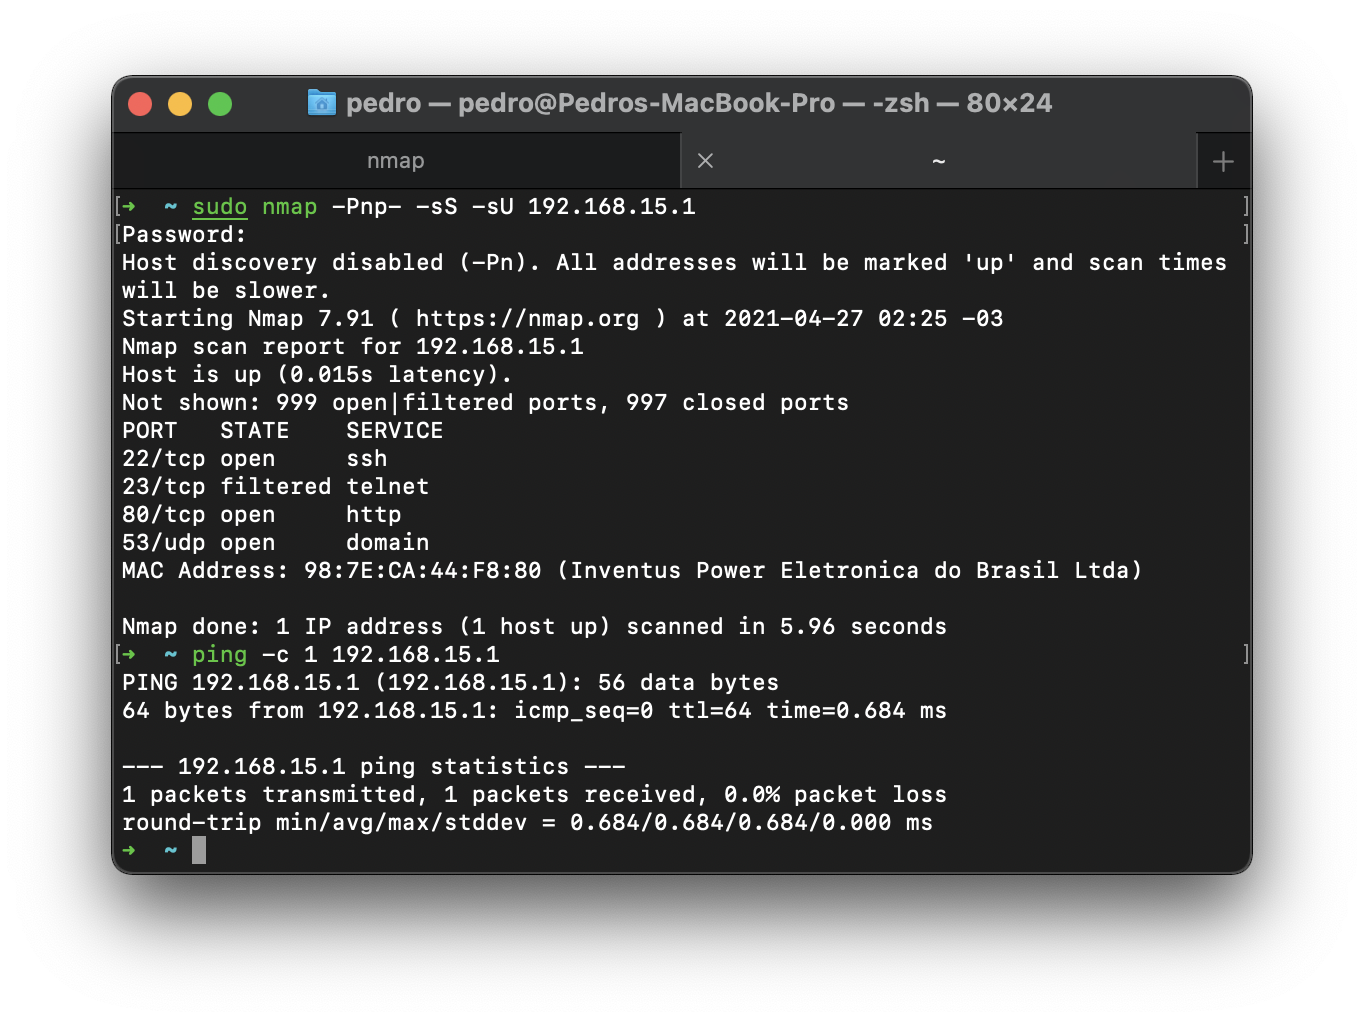
\includegraphics[width=\linewidth]{contents/cpes-and-research-data/allowed-ingress-traffic/cpe-allowed-ingress-traffic.png}
    \caption{\gls{cpe} Allowed Ingress Traffic}
    \label{figure:cpe_allowed_ingress_traffic}
\end{figure}

Then, to detect the ports exposed to the broadband network, the \gls{cpe} had to be connected to the copper or fiber cable of the \gls{isp} to acquire a public \gls{ip} address. The tools were executed from a device on the \gls{wan}, directing the scan to the \gls{cpe}’s public \gls{ip}.

Table \ref{table:cpes_ingress} presents all ingress traffic allowed by the \gls{cpe} on both \gls{lan} and \gls{wan} sides.

\begin{table}[h]
    \makebox[\linewidth]{
        \begin{tabular}{c|c|c}
            \thead{\gls{cpe} Identifier} & \thead{From \gls{lan}-side} & \thead{From \gls{wan}-side} \\
            \hline
            \gls{cpe}-0 & \texttt{53/udp 80/tcp 443/tcp 5431/tcp \gls{icmp}} & \texttt{7547/tcp \gls{icmp}} \\
            \gls{cpe}-1 & \texttt{53/udp 80/tcp 443/tcp 5431/tcp \gls{icmp}} & \texttt{7547/tcp \gls{icmp}} \\
            \gls{cpe}-2 & \texttt{22/tcp 53/udp 80/tcp \gls{icmp}} & \texttt{22/tcp 80/tcp 7547/tcp \gls{icmp}} \\
            \gls{cpe}-3 & \texttt{22/tcp 53/udp 80/tcp \gls{icmp}} & \texttt{22/tcp 80/tcp 7547/tcp \gls{icmp}} \\
            \gls{cpe}-4 & \texttt{53/udp 80/tcp \gls{icmp}} & \texttt{7547/tcp \gls{icmp}} \\
            \gls{cpe}-5 & \texttt{53/udp 80/tcp \gls{icmp}} & \texttt{7547/tcp \gls{icmp}} \\
            \gls{cpe}-6 & \texttt{80/tcp 443/tcp \gls{icmp}} & \texttt{7547/tcp \gls{icmp}} \\
            \gls{cpe}-7 & \texttt{53/udp 80/tcp 5555/tcp \gls{icmp}} & \texttt{7547/tcp \gls{icmp}} \\
        \end{tabular}
    }
    \caption{Allowed Ingress Traffic of the \gls{cpe}s}
    \label{table:cpes_ingress}
\end{table}

\FloatBarrier

\subsection{Outgoing Traffic}

\glspl{cpe} 4 and 7 have tcpdump \cite{tcpdump} installed, allowing the outgoing traffic to be inspected from inside the device. The tcpdump binary was introduced on \gls{cpe} 5 via a \gls{tftp} server \cite{rfc1350}, allowing the traffic to be inspected as well.

\glspl{cpe} 0 to 3 and 6 neither have tcpdump installed nor are able to have it introduced on them by any means. On \glspl{cpe} 0 and 1, the only data that could be extracted were snapshots of the \gls{tcp} Translation Table.

With the environment set, the capture is started and the broadband connection is provided to the \gls{cpe}, allowing it to initiate connections.

\subsubsection{CWMP}

On all \glspl{cpe} was observed \gls{cwmp} traffic to the \gls{isp} \gls{acs} in a very similar pattern. The default configuration points to an intermediary \gls{acs} with hardcoded credentials. Table \ref{table:cpes_acs_hardcoded} presents all different configurations found on the \gls{cpe}s.

\begin{table}[h]
    \makebox[\linewidth]{
        \begin{tabular}{c|c|c}
            \thead{\gls{acs} \gls{url}} & \thead{\gls{acs} Username} & \thead{\gls{acs} Password} \\
            \hline
            \url{http://acs.telesp.net.br:7005/cwmpWeb/WGCPEMgt} & \texttt{mitrastar} & \texttt{telefonica} \\
            \url{http://acs.telesp.net.br:7005/cwmpWeb/WGCPEMgt} & \texttt{acsclient} & \texttt{telefonica} \\
            \url{https://acs.gvt.net.br} & \texttt{acsclient} & \texttt{acsvivo15sca} \\
            \url{https://acs.gvt.net.br} & \texttt{acsclient} & \texttt{acsgvt25sca} \\
        \end{tabular}
    }
    \caption{Hardcoded \gls{acs} Credentials of the \gls{cpe}s}
    \label{table:cpes_acs_hardcoded}
\end{table}

The \gls{cpe} sends a \gls{cwmp} Inform request that is answered with an \gls{acs} request for changing Connection Request Credentials and enabling Periodic Inform with an interval of 108000 seconds. The new Connection Request username set by the \gls{acs} is a combination of \gls{cpe} Serial Number, \gls{cpe} Product Class, and \gls{cpe} \gls{oui}, respectively concatenated with a dash used as a separator. The password is a 128-bit number encoded as a hexadecimal string, likely the \gls{md5} hash of an unknown value. A new password is issued everytime that the \gls{cpe} registers itself using the default \gls{cwmp} settings. Table \ref{table:cpes_connreq} presents the credentials acquired by each \gls{cpe} in one of the registrations with the default \gls{acs}.

\begin{table}[h]
    \makebox[\linewidth]{
        \begin{tabular}{c|c|c}
            \thead{\gls{cpe} Identifier} & \thead{Connection Request Username} & \thead{Connection Request Password} \\
            \hline
            \gls{cpe}-0 & \texttt{5CC9D3D8731B-RTA9227W-D112-C0D962} & \texttt{4f6a306dc705bab62a07415460231bec} \\
            \gls{cpe}-1 & \texttt{542F8A6CBE99-RTV9015VW-C0D962} & \texttt{b10f38755e844832aa586ccca67572b7} \\
            % \gls{cpe}-2 & \texttt{} & \texttt{} \\
            % \gls{cpe}-3 & \texttt{} & \texttt{} \\
            \gls{cpe}-4 & \texttt{1072230D83CC-RTF3505VW-N2-009096} & \texttt{7f6fc3cb94341ace99154184e71cd0eb} \\
            \gls{cpe}-5 & \texttt{987ECA44F881-RTF8115VW-009096} & \texttt{da9e89b37c32650c44c826db21f54bc8} \\
            % \gls{cpe}-6 & \texttt{} & \texttt{} \\
            % \gls{cpe}-7 & \texttt{} & \texttt{} \\
        \end{tabular}
    }
    \caption{Connection Request Credentials of the \gls{cpe}s}
    \label{table:cpes_connreq}
\end{table}

After performing the requested changes and notifying the \gls{acs} about it, the \gls{acs} now requests the \gls{acs} \gls{url} and Credentials to be changed. The final \gls{acs} used by all \glspl{cpe} is the same. It was verified that the username and passwords used to access the \gls{acs} are the UNIX Timestamp of the time that the credentials were issued, respectively appended by characters `u` and `a`, as presented in Table \ref{table:cpes_acs_assigned}.

\begin{table}[h]
    \makebox[\linewidth]{
        \begin{tabular}{c|c|c}
            \thead{\gls{acs} \gls{url}} & \thead{\gls{acs} Username} & \thead{\gls{acs} Password} \\
            \hline
            \url{http://acs.telesp.net.br:7015/cwmpWeb/CPEMgt} & \texttt{\$\{UNIX\_TIMESTAMP\}u} & \texttt{\$\{UNIX\_TIMESTAMP\}a} \\
        \end{tabular}
    }
    \caption{Assigned \gls{acs} Credentials of the \gls{cpe}s}
    \label{table:cpes_acs_assigned}
\end{table}

A \gls{cwmp} Inform request is sent to the new \gls{acs}. If the device was running an outdated firmware at the time of the request, the \gls{acs} will respond if a \gls{cwmp} Download request with the Firmware Upgrade Image. In all cases, the firmware image was hosted under \url{http://201.95.254.33:18273/fileserver/}. The server seems to be accessible only from an \gls{ip} address that belongs to the \gls{isp}, other addresses experience timeouts when requesting data.

\FloatBarrier

\subsection{VoIP}

To configure the \gls{voip} service on the \gls{crg}s, a similar process to the manual Internet setup is followed on both equipment. There is no difference in this process on copper-based and fiber-based devices.

The \gls{sip} configuration collected from all \glspl{cpe} show that an outbound proxy is always used. This proxy is located at \url{192.168.80.1} and is only accessible on a network with \gls{vlan} \gls{id} different from the one used for the Internet Connection.

\begin{figure}[h]
    \centering
    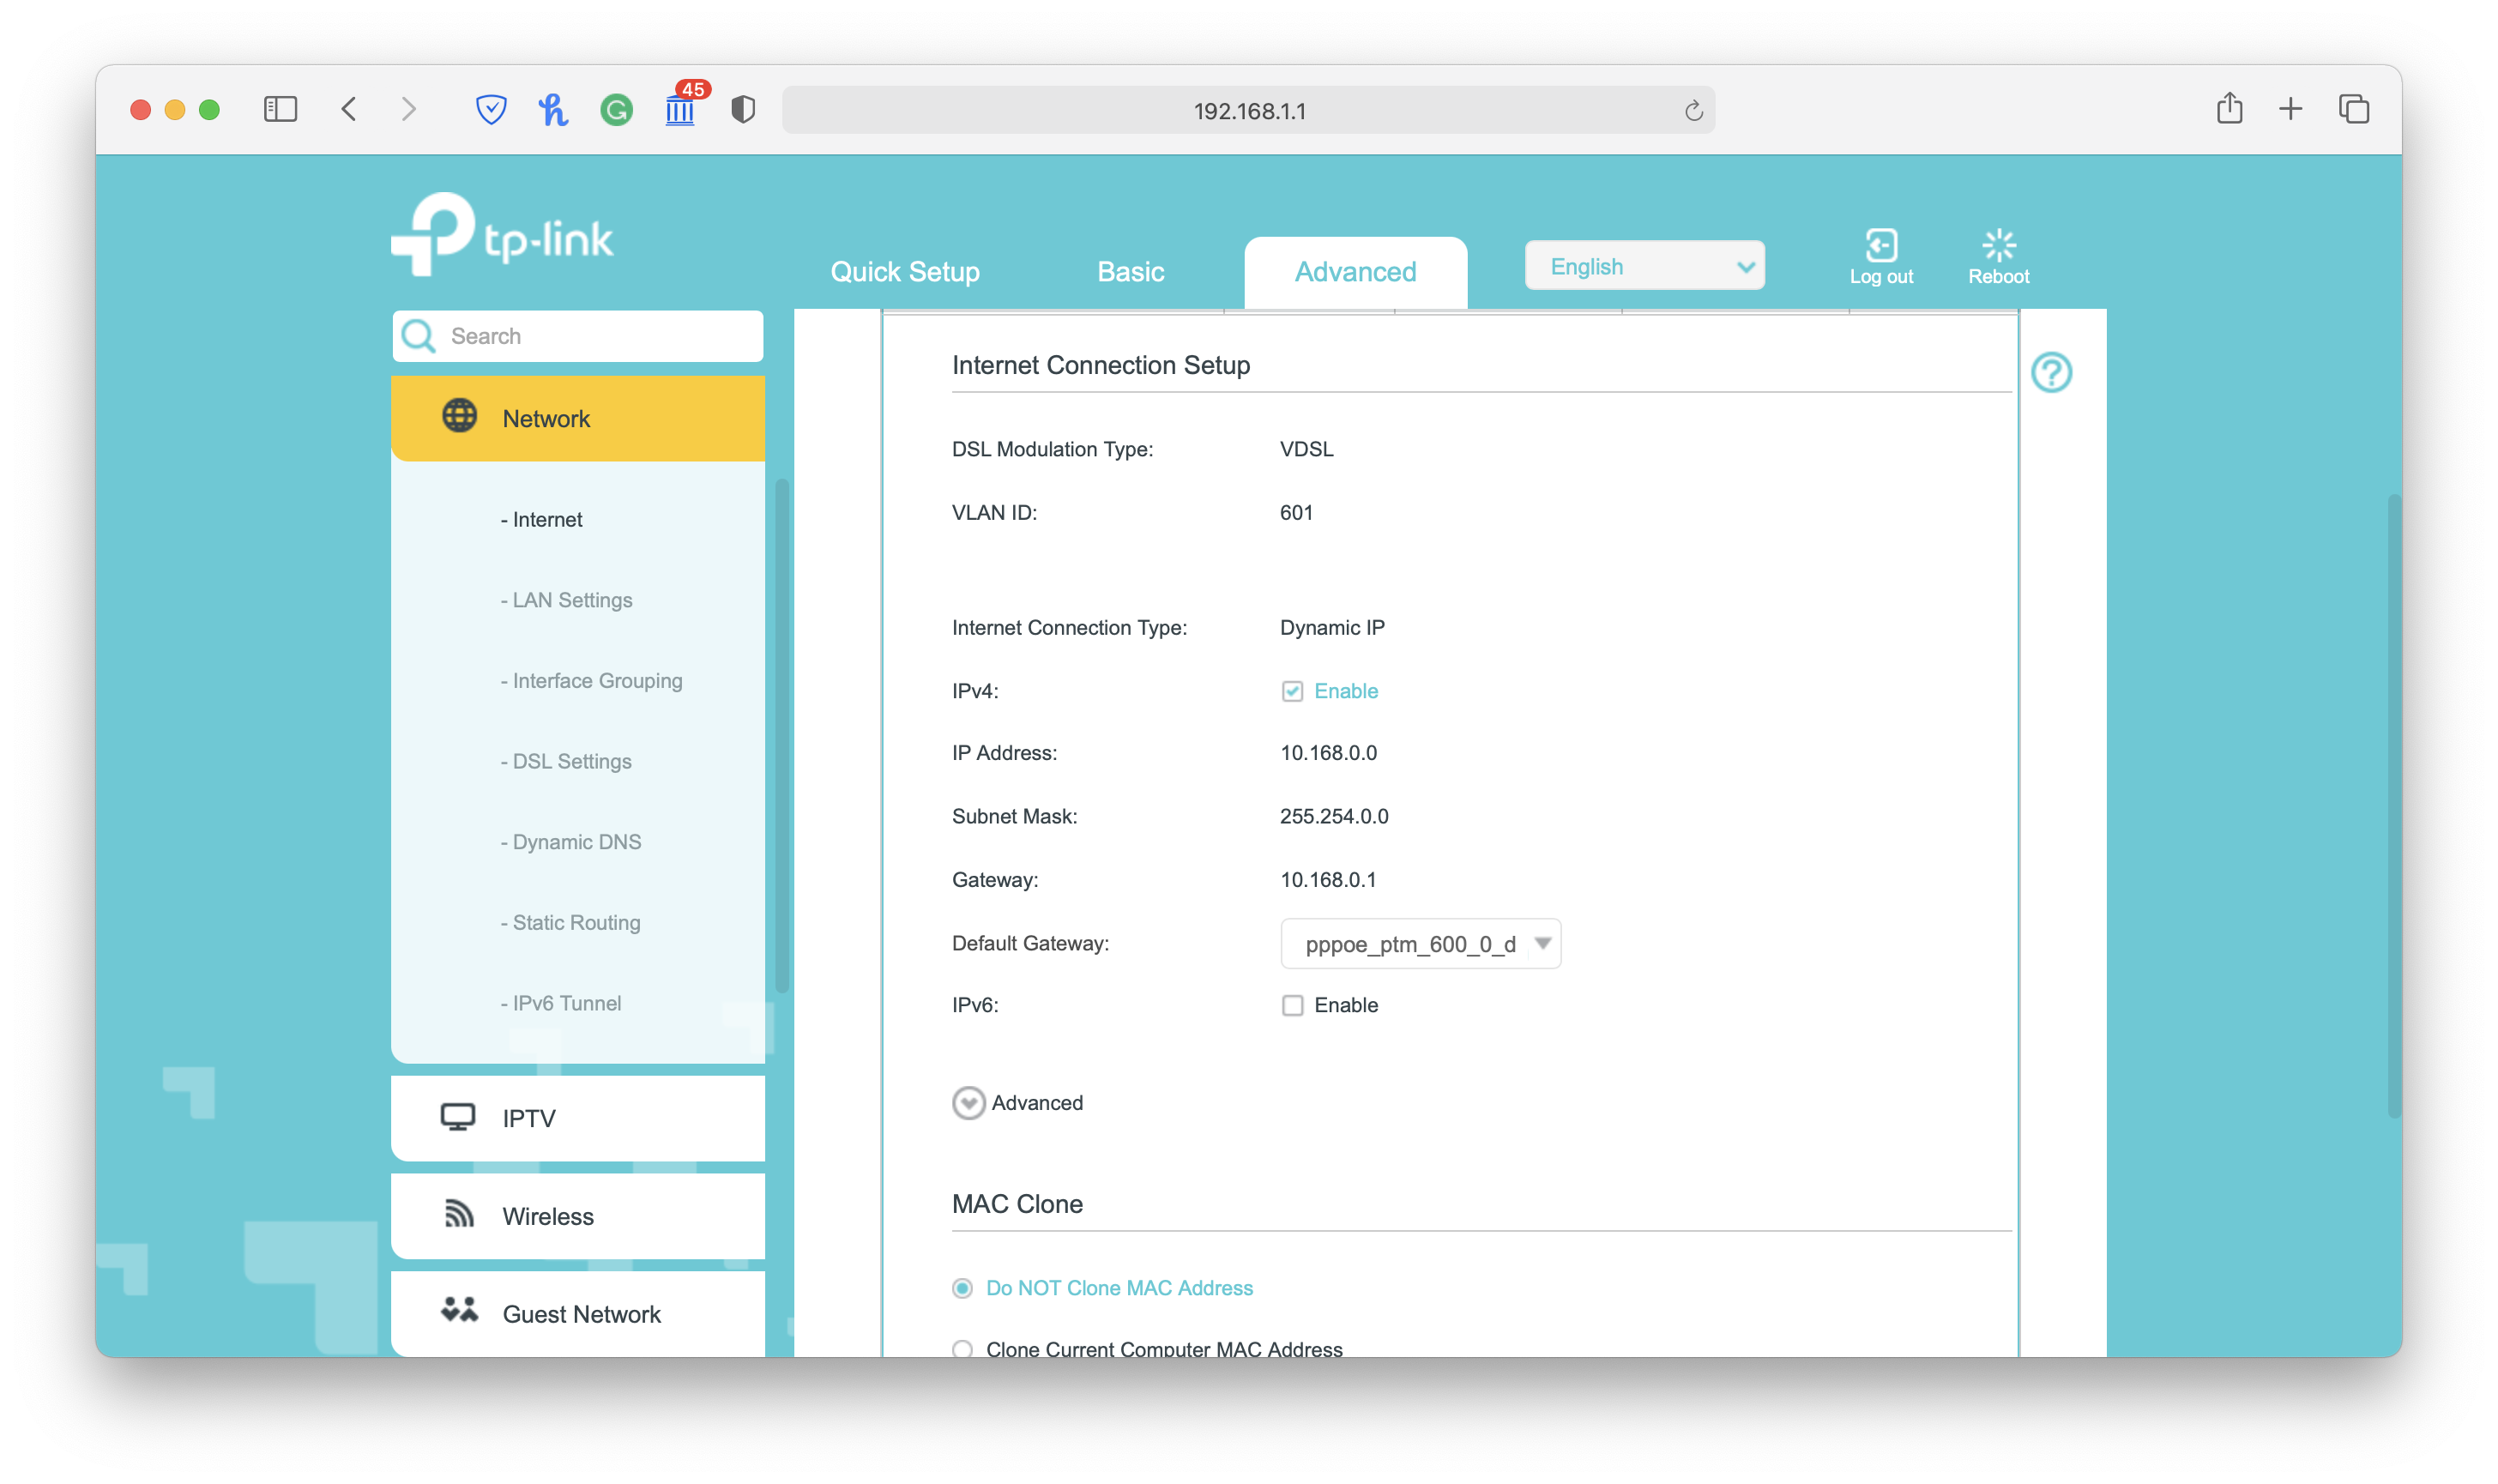
\includegraphics[width=\linewidth]{contents/substituting-the-isp-cpe/voip/advanced-network-internet-vlan601.png}
    \caption{\gls{vlan} 601 Settings of the \gls{crg}s}
    \label{figure:crgs_vlan601}
\end{figure}

Then, the Internet Configuration page must be accessed and a new connection created. The \gls{vlan} \gls{id} must be set to 601 and the Connection Type to Dynamic \gls{ip}, as shown in Figure \ref{figure:crgs_vlan601}. The default gateway must not be changed and \gls{ip}v6 must not be enabled.

After creating this new connection, an \gls{ip} address is automatically acquired. The joined network is part of the \url{10.0.0.0/8} \gls{ip}v4 range and doesn’t provide access to the Internet.

\begin{figure}[h]
    \centering
    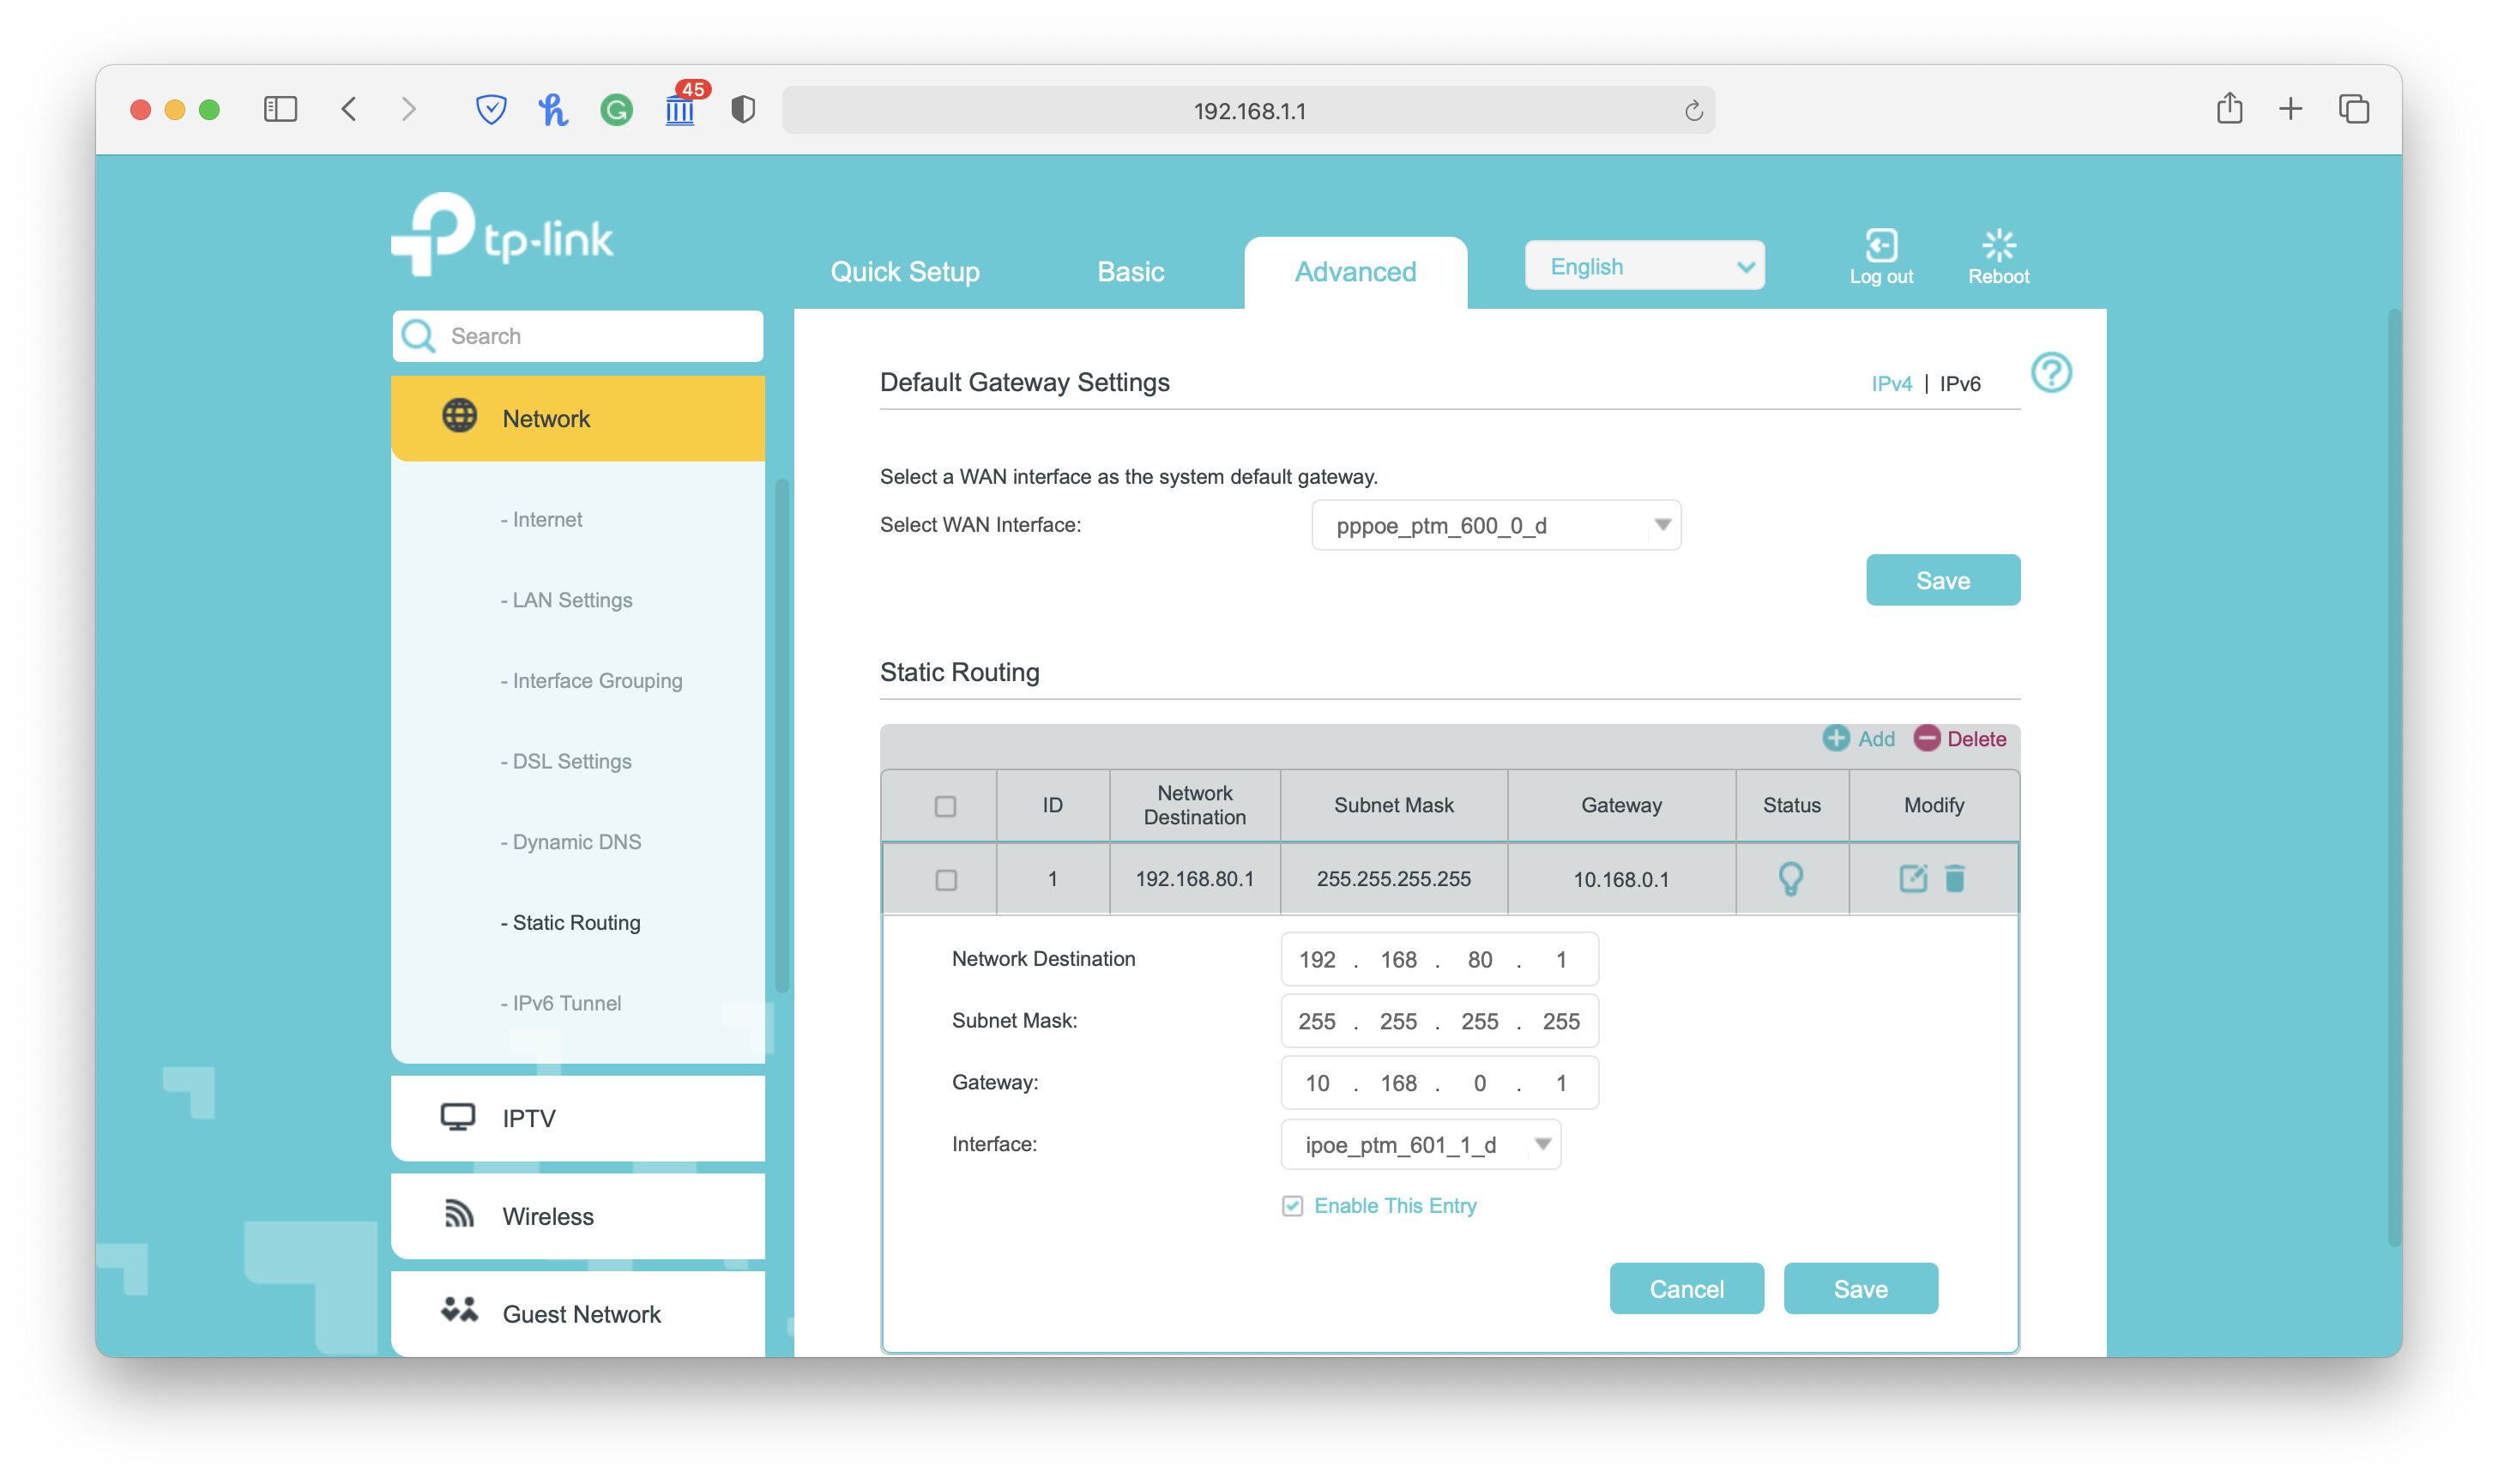
\includegraphics[width=\linewidth]{contents/substituting-the-isp-cpe/voip/advanced-network-staticrouting.png}
    \caption{Static Routing Settings of the \gls{crg}s}
    \label{figure:crgs_staticrouting}
\end{figure}

As the default gateway is set to the Internet Connection previously configured, a static route must be configured to make connections to the \gls{sip} Proxy be routed to the new network. This can also be done on the advanced section of the management interface. The Network Destination and Subnet Mask must be respectively set to \url{192.168.80.1} and \url{255.255.255.255}. The gateway field must be filled with the \gls{ip} address of the gateway assigned to the device on the network with \gls{vlan} \gls{id} 601, and the interface must point to the same network as well, as shown in Figure \ref{figure:crgs_staticrouting}. The experiments show that even after 6 months and reboots, the gateway assigned never changes, allowing the static route not be reconfigured when a new connection is established.

\begin{figure}[h]
    \centering
    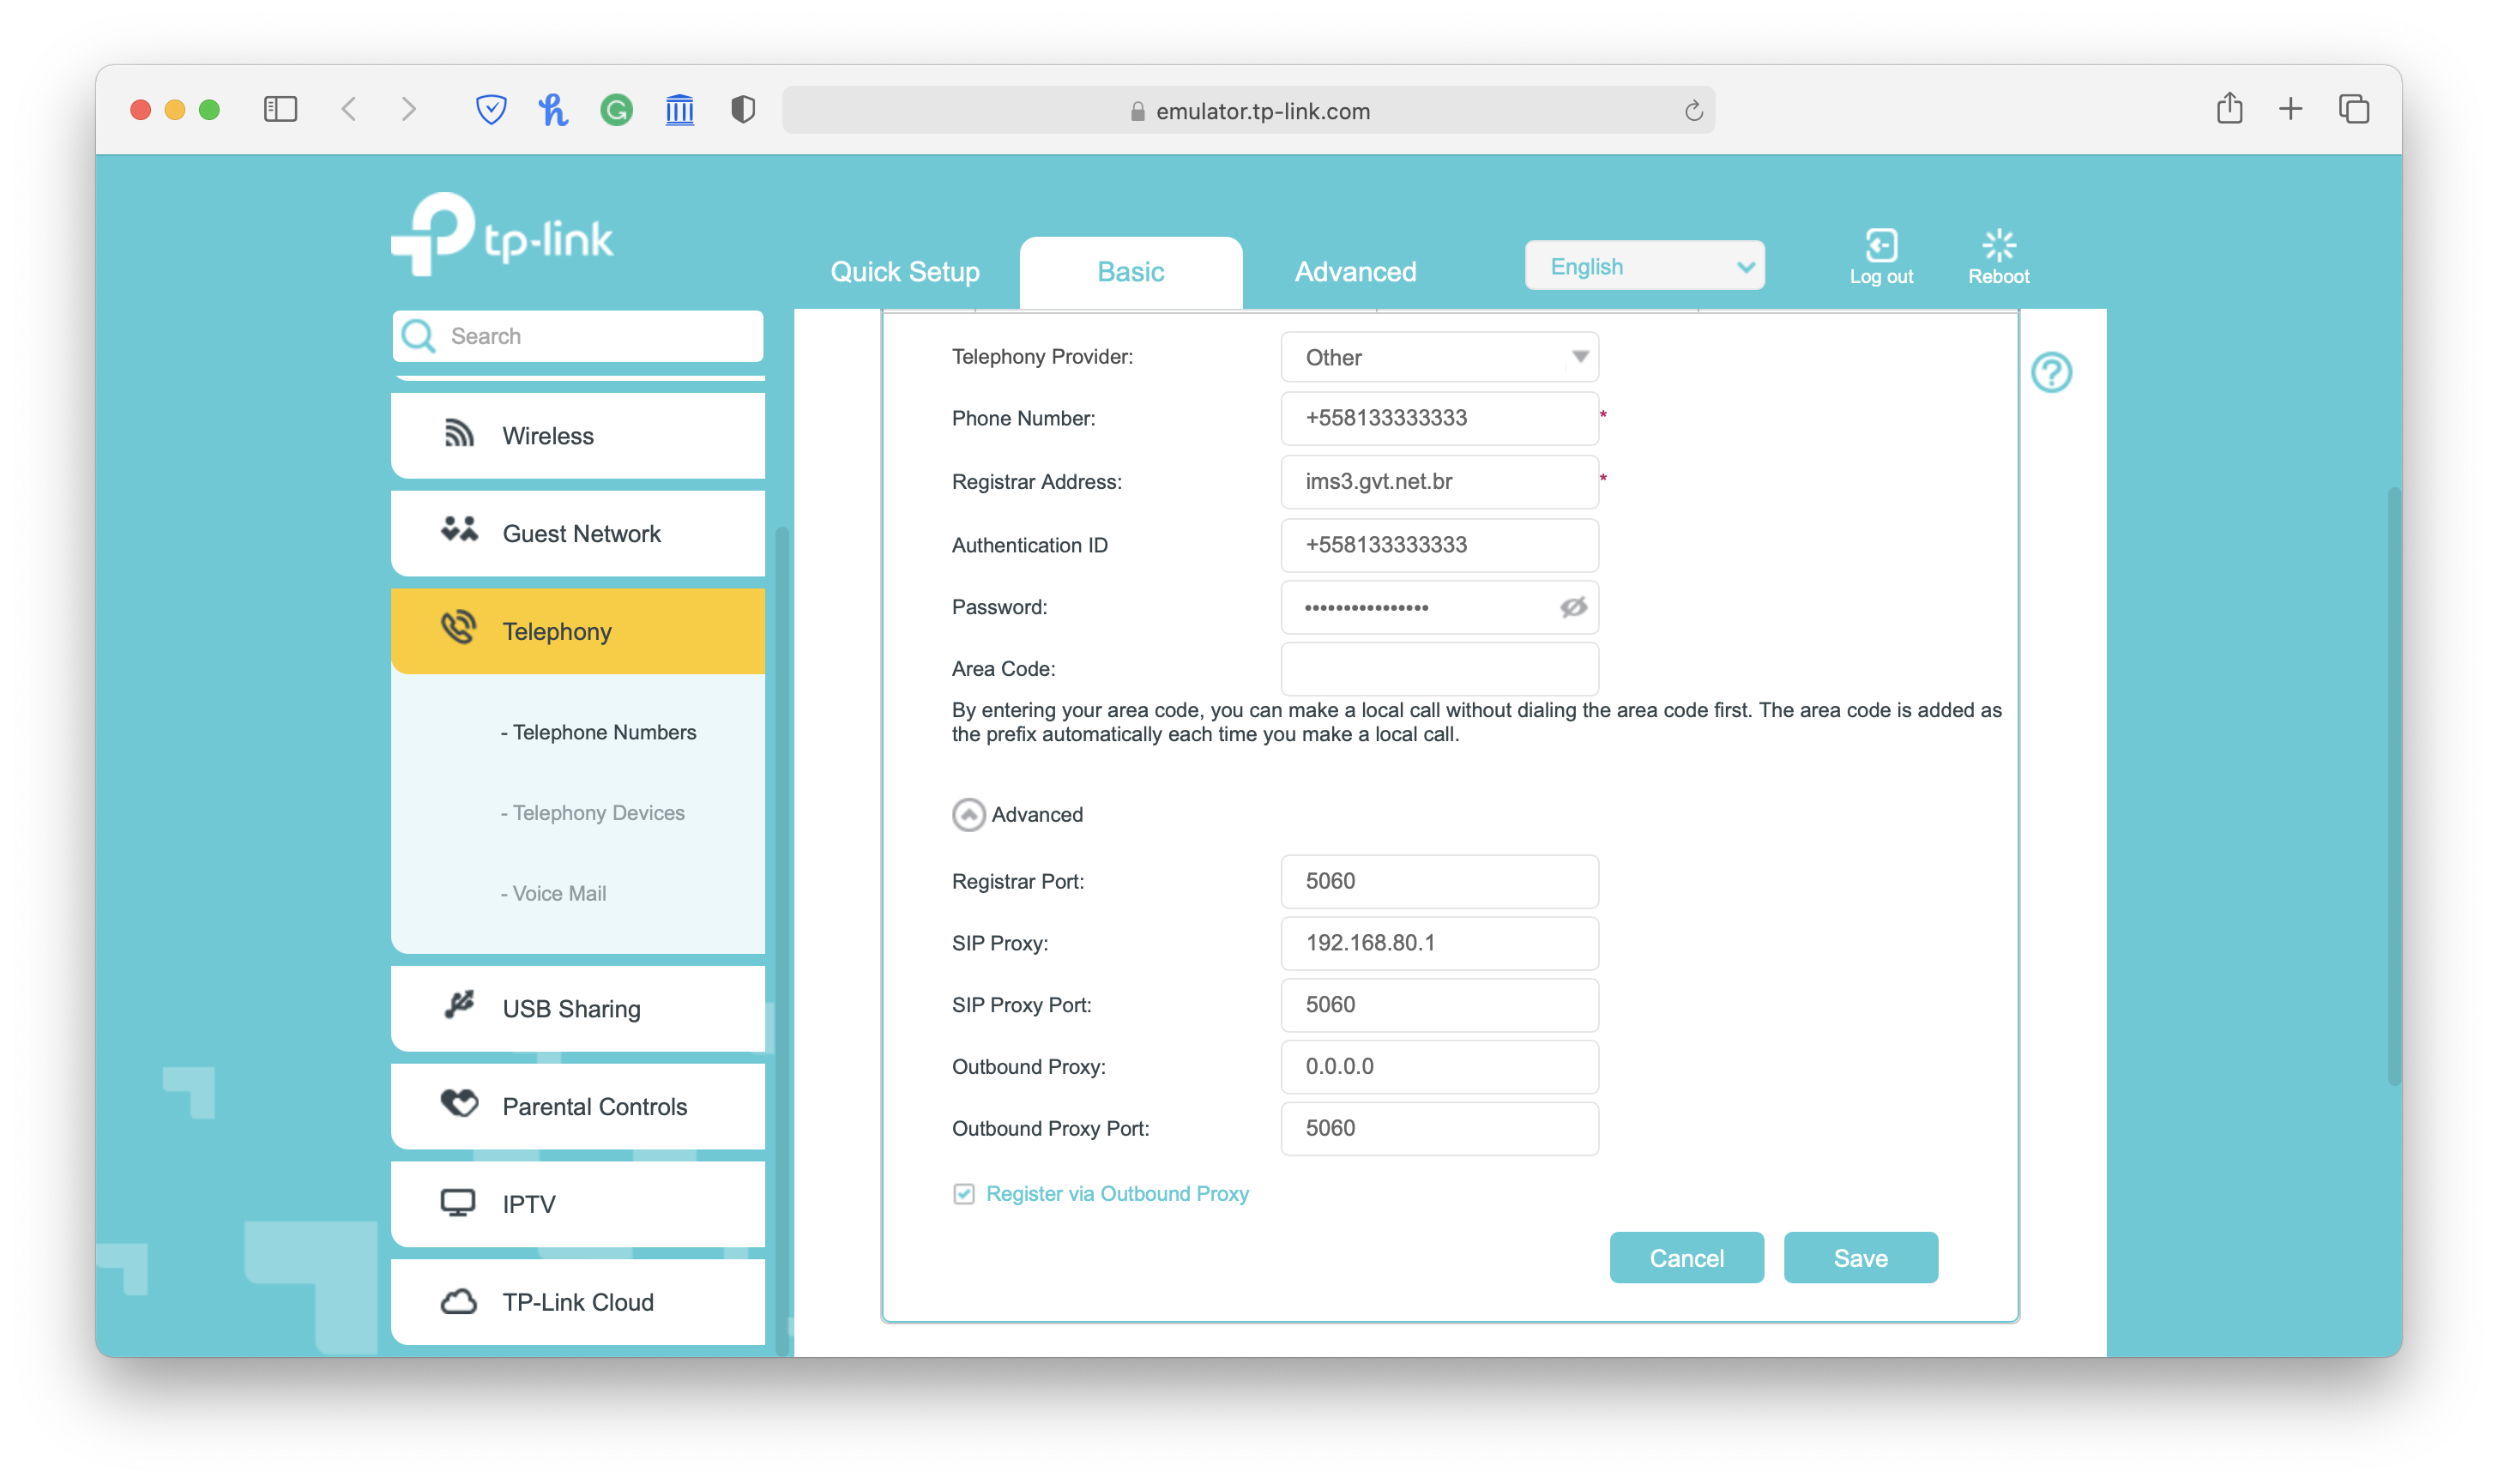
\includegraphics[width=\linewidth]{contents/substituting-the-isp-cpe/voip/basic-telephony-telephonenumbers.png}
    \caption{Telephone Numbers Settings of the \gls{crg}s}
    \label{figure:crgs_telephonenumbers}
\end{figure}

With the \gls{voip} Connection configured, a \gls{sip} client can be configured on the \gls{crg} itself, allowing analog telephones to work when connected to the \gls{rj11} ports. On the basic section of the \gls{http} Management Interface, telephone numbers can be registered. The Phone Number and Authentication \gls{id} must be set to the customer’s phone number formatted following the E.164 standard. The Registrar Address and Password are set to the values acquired from the \gls{isp} \gls{cpe} originally used by the customer. Finally, the Outbound Proxy is set to \url{192.168.80.1}, keeping the Outbound Proxy Port value of 5060 and the Register via Outbound Proxy checkbox enabled. The settings are shown in Figure \ref{figure:crgs_telephonenumbers}.

After the phone number was properly registered, the connection status showed a blue check. An analog phone was connected to the \gls{rj11} port and a number was dialed. Unfortunately the connection was unreliable, sometimes the call was successful, but most of the time there was a problem. The dialer could listen but could not be heard, the opposite also happened. After hanging a call, the number could not receive or make calls for some minutes. The phone rang indefinitely, even when out of the hook.

To diagnose the problem, a \gls{sip} client was used on a computer instead of using the \gls{crg} one. This should work fine, because differently from the \gls{isp} \gls{cpe}s, the \gls{crg} is not configured to block connections going to the \gls{sip} proxy. The Telephone app was used as \gls{sip} client, as it was free and open source. But after setting the connection on it, similar problems arose.

As it was unlikely that both \gls{sip} clients were not properly implemented, the \gls{sip} traffic of the \gls{crg} the the client running on the computer were captured and compared with the traffic previously captured from the \gls{sip} \gls{cpe}. Everything looked very similar but with one subtle difference, the \gls{sip} clients from the \gls{crg} and the computer were sending keep-alive requests to the \gls{sip} server, while the \gls{cpe} wasn’t sending them.

Looking at the implementation of the computer and \gls{crg} clients, it was found that they use the PJSIP to establish and manage the \gls{sip} connection. The \gls{crg} used the PJSIP \gls{cli}, while the computer client used the PJSIP library. Both are configured by default to send \gls{cr}-\gls{lf} as keep-alive packets every 15 seconds.

The Telephone app is recompiled with a configuration that prevents those keep-alive requests from being sent. After doing that, the \gls{sip} client started to work perfectly, just like the \gls{sip} \gls{cpe}, confirming the problem was indeed the keep-alive packets.

Unfortunately the \glspl{crg} have no configuration that allows keep-alive to be disabled. Additionally, the PJSUA \gls{cli} doesn’t have this flag either, so the PJSUA library should be used instead to allow this configuration to be changed. The firmware of the devices are closed-source, so it is not easy to build a new firmware with the changes required.

While looking for alternatives, it was found that both \glspl{crg} have iptables installed on them and have the necessary modules installed to filter the keep-alive packages going to the \gls{sip} proxy. The devices were restarted without the copper or fiber cables connected to them, preventing any connection from being established. Then the \gls{ssh} Management Interface was accessed and iptables rule was created, dropping the \gls{sip} keep-alive packets. The copper and fiber cables were reconnected and the connection established. From that point, although the \gls{sip} client was still sending the problematic packets, the \gls{sip} server never received them and the service started working just like the modified Telephone app.

\begin{lstlisting}[language=Bash,numbers=left]
iptables -I OUTPUT -p udp -j DROP -d 192.168.80.1 -m udp --dport 5060 -m string --hex-string '|0d0a|' --algo bm --from 28 --to 30
\end{lstlisting}

The solution found is untethered and the processed needs to be executed every time the \gls{crg} reboots. But it is feasible to use if the device is not rebooted frequently, or if a computer that is always connected to it via a wired connection is able to automatically execute the process every time the connection is lost and then reestablished. Another possibility would be having the \gls{sip} proxy point to a device that drops the keep-alive packets and then forward to the real \gls{sip} proxy.

It is important to notice that the \gls{crg} doesn’t need to support \gls{voip} if a \gls{sip} client running on another device can be used in the desired scenario, it just needs to be able to establish a connection with the proper \gls{vlan} \gls{id} and Connection Type. This also means that consumers can acquire cheaper \glspl{crg} that don’t have \gls{voip} built-in and use other solutions that fit in the use-case, like an external \gls{ata}.

\FloatBarrier

\subsection{IPTV}

As previously mentioned, the test environments didn’t have an \gls{iptv} subscription of the \gls{isp}, but information the data collected indicates how it could be properly configured. Although problems like the \gls{sip} keep-alive packets wouldn’t be detected.

\begin{figure}[h]
    \centering
    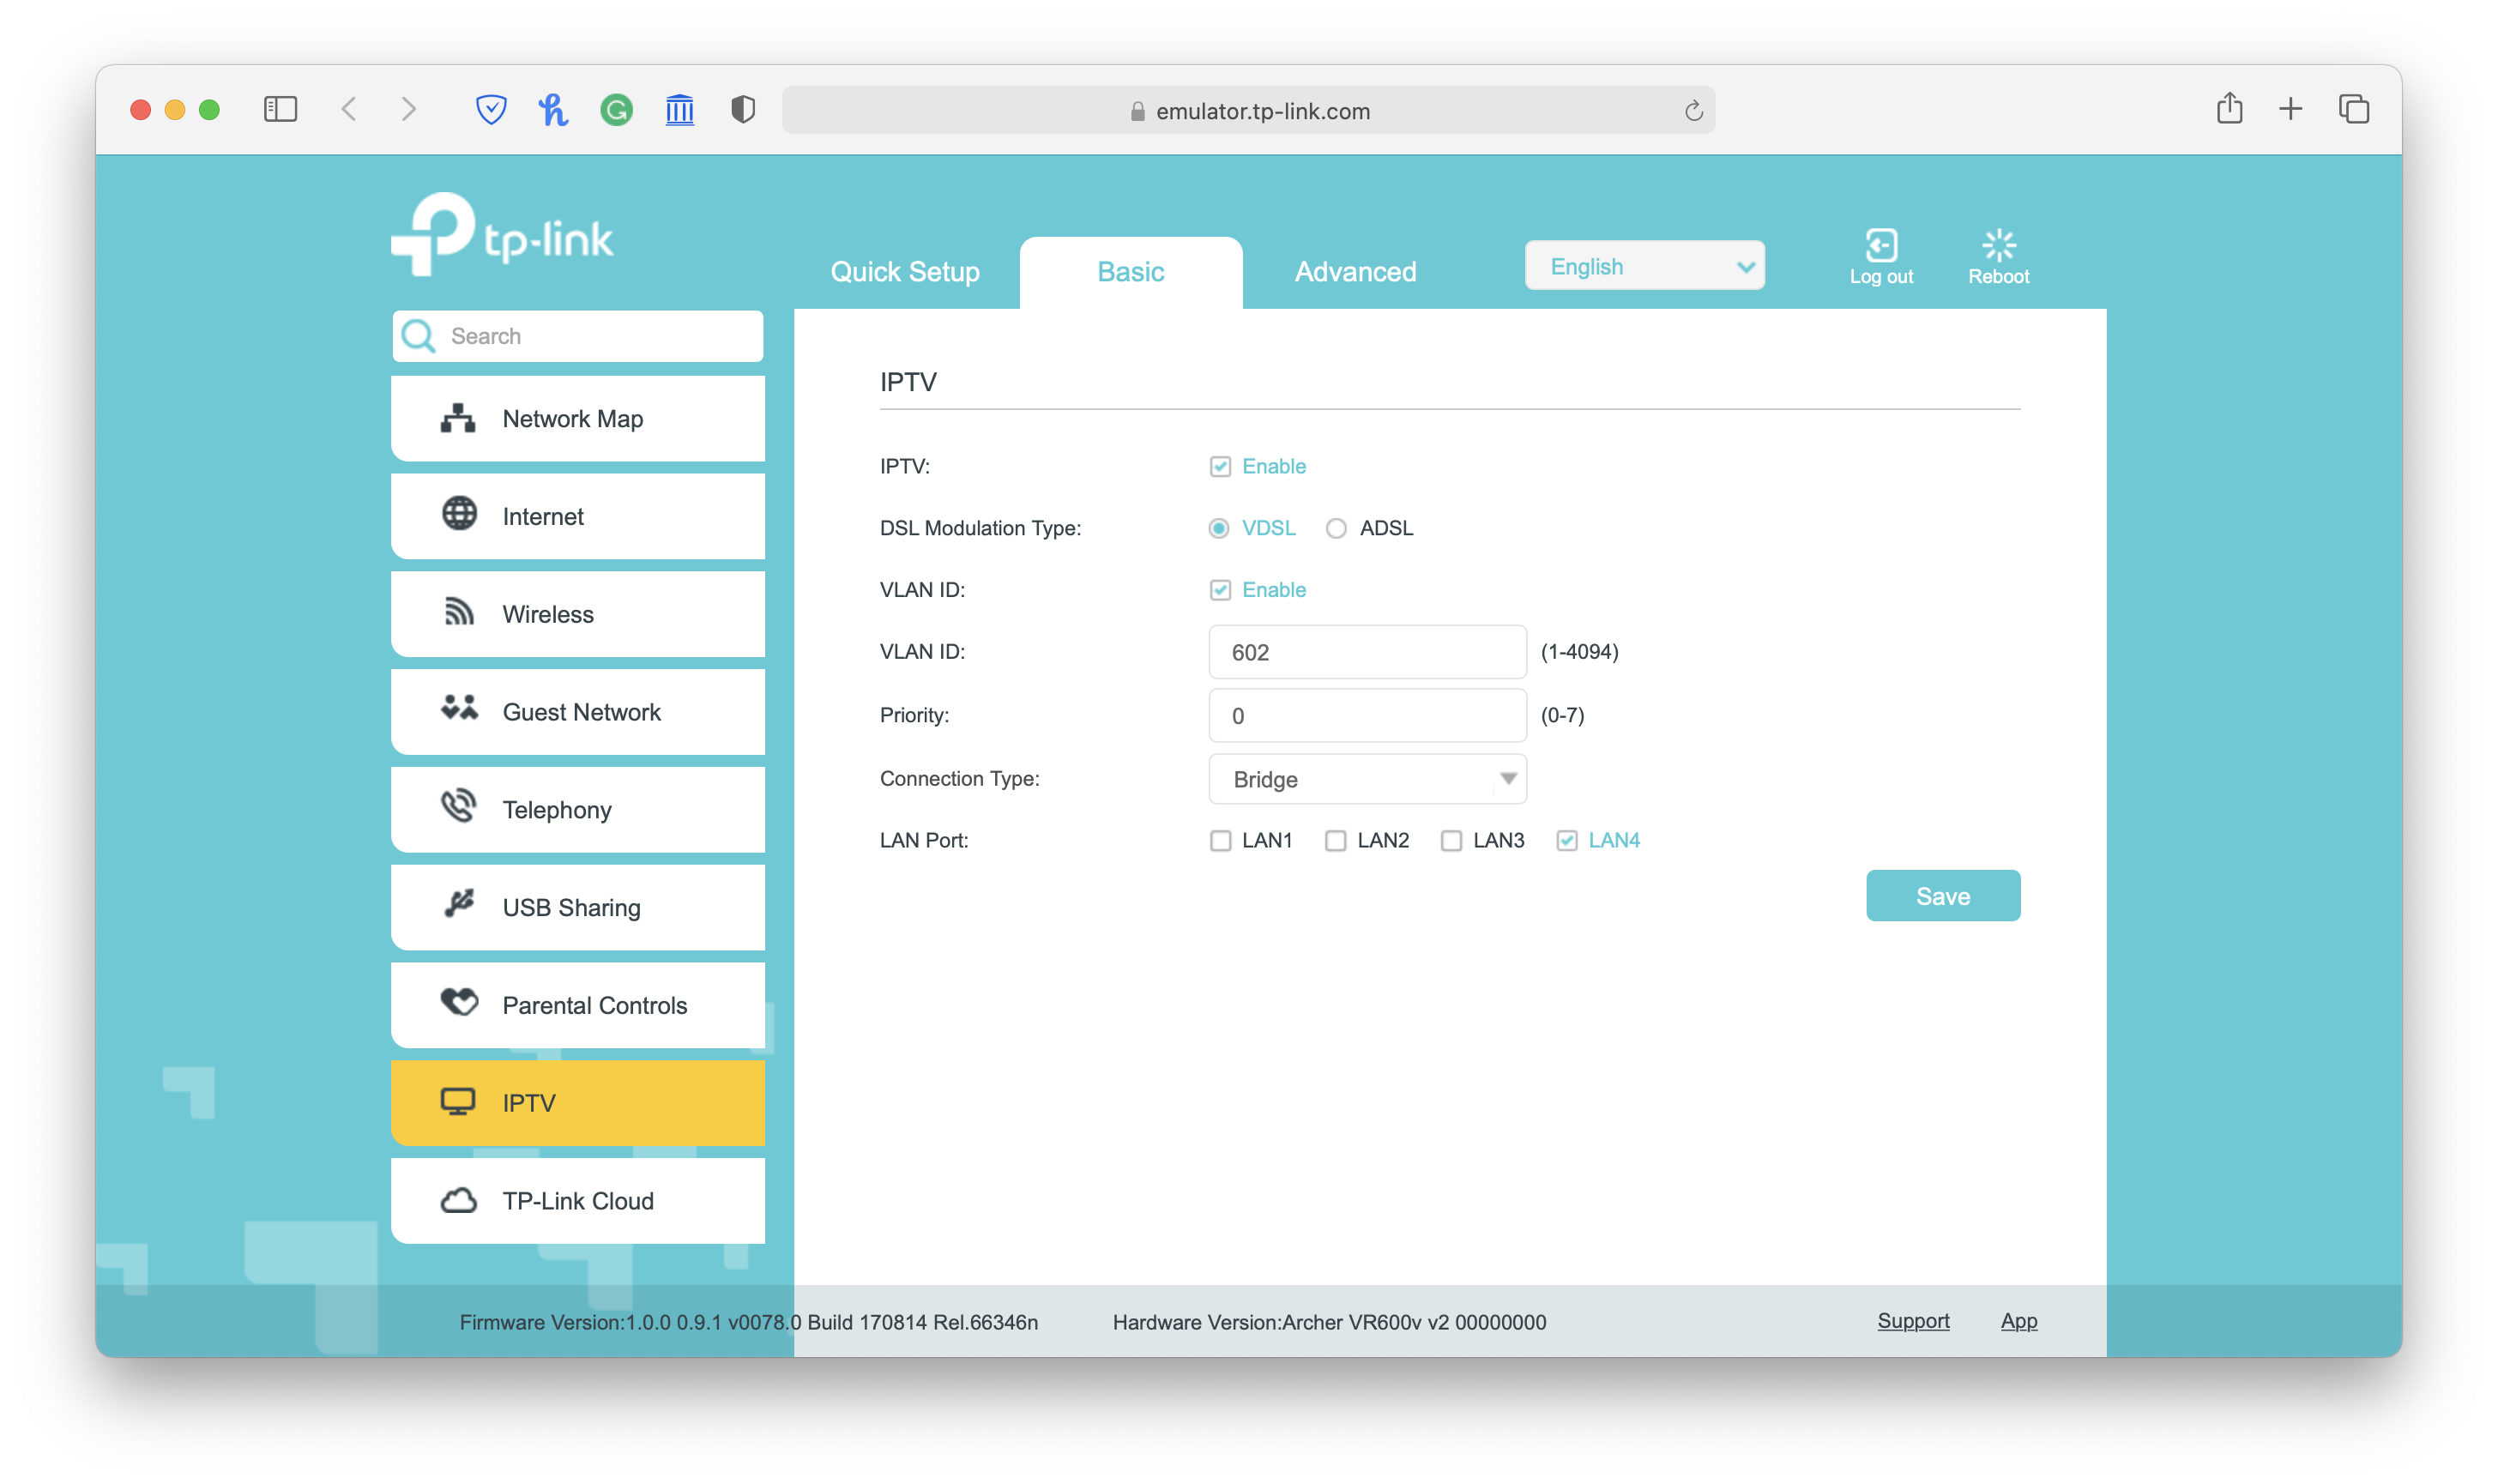
\includegraphics[width=\linewidth]{contents/substituting-the-isp-cpe/iptv/basic-iptv.png}
    \caption{\gls{iptv} Settings of the \gls{crg}s}
    \label{figure:crgs_iptv}
\end{figure}

The \gls{iptv} traffic is routed through a third network. This can be configured on the basic section of the \gls{http} Management Interface, as shown on Figure \ref{figure:crgs_iptv}. \gls{iptv} is enabled, the \gls{vlan} \gls{id} is set 602, and the Connection Type kept as Bridge. The set-top box provided by the \gls{isp} is connected to a \gls{lan} port of the residential gateway through an Ethernet cable. That specific \gls{lan} port must be checked on the configuration page of \gls{iptv}, allowing the \gls{stb} to access the correct \gls{vlan}.

This should be enough to have the \gls{iptv} service properly working, unfortunately it wasn’t verifiable and additional tweaking may be required.

\FloatBarrier


\subsection{Anonymously Accessing Management Interfaces}

All devices have their \gls{http} Management Interface enabled by default and can be accessed by navigating to \url{http://192.168.15.1} on a browser. This interface provides information about the \gls{cpe} and its network.

On the main page, Figure \ref{figure:main_page_cpe_http_management_interface}, both public and private \gls{ip} addresses of the device can be viewed together with the gateway and \gls{dns} servers configured. The \gls{ssid}, security protocol, \gls{wps} state, and channel of the wireless networks are specified, also showing which \gls{lan} ports are in use. A list with the hostname, \gls{mac} address, and \gls{ip} of all wired and wireless clients currently connected to the \gls{cpe} is present. If \gls{voip} is configured, the telephone number is shown.

\begin{figure}[h]
    \centering
    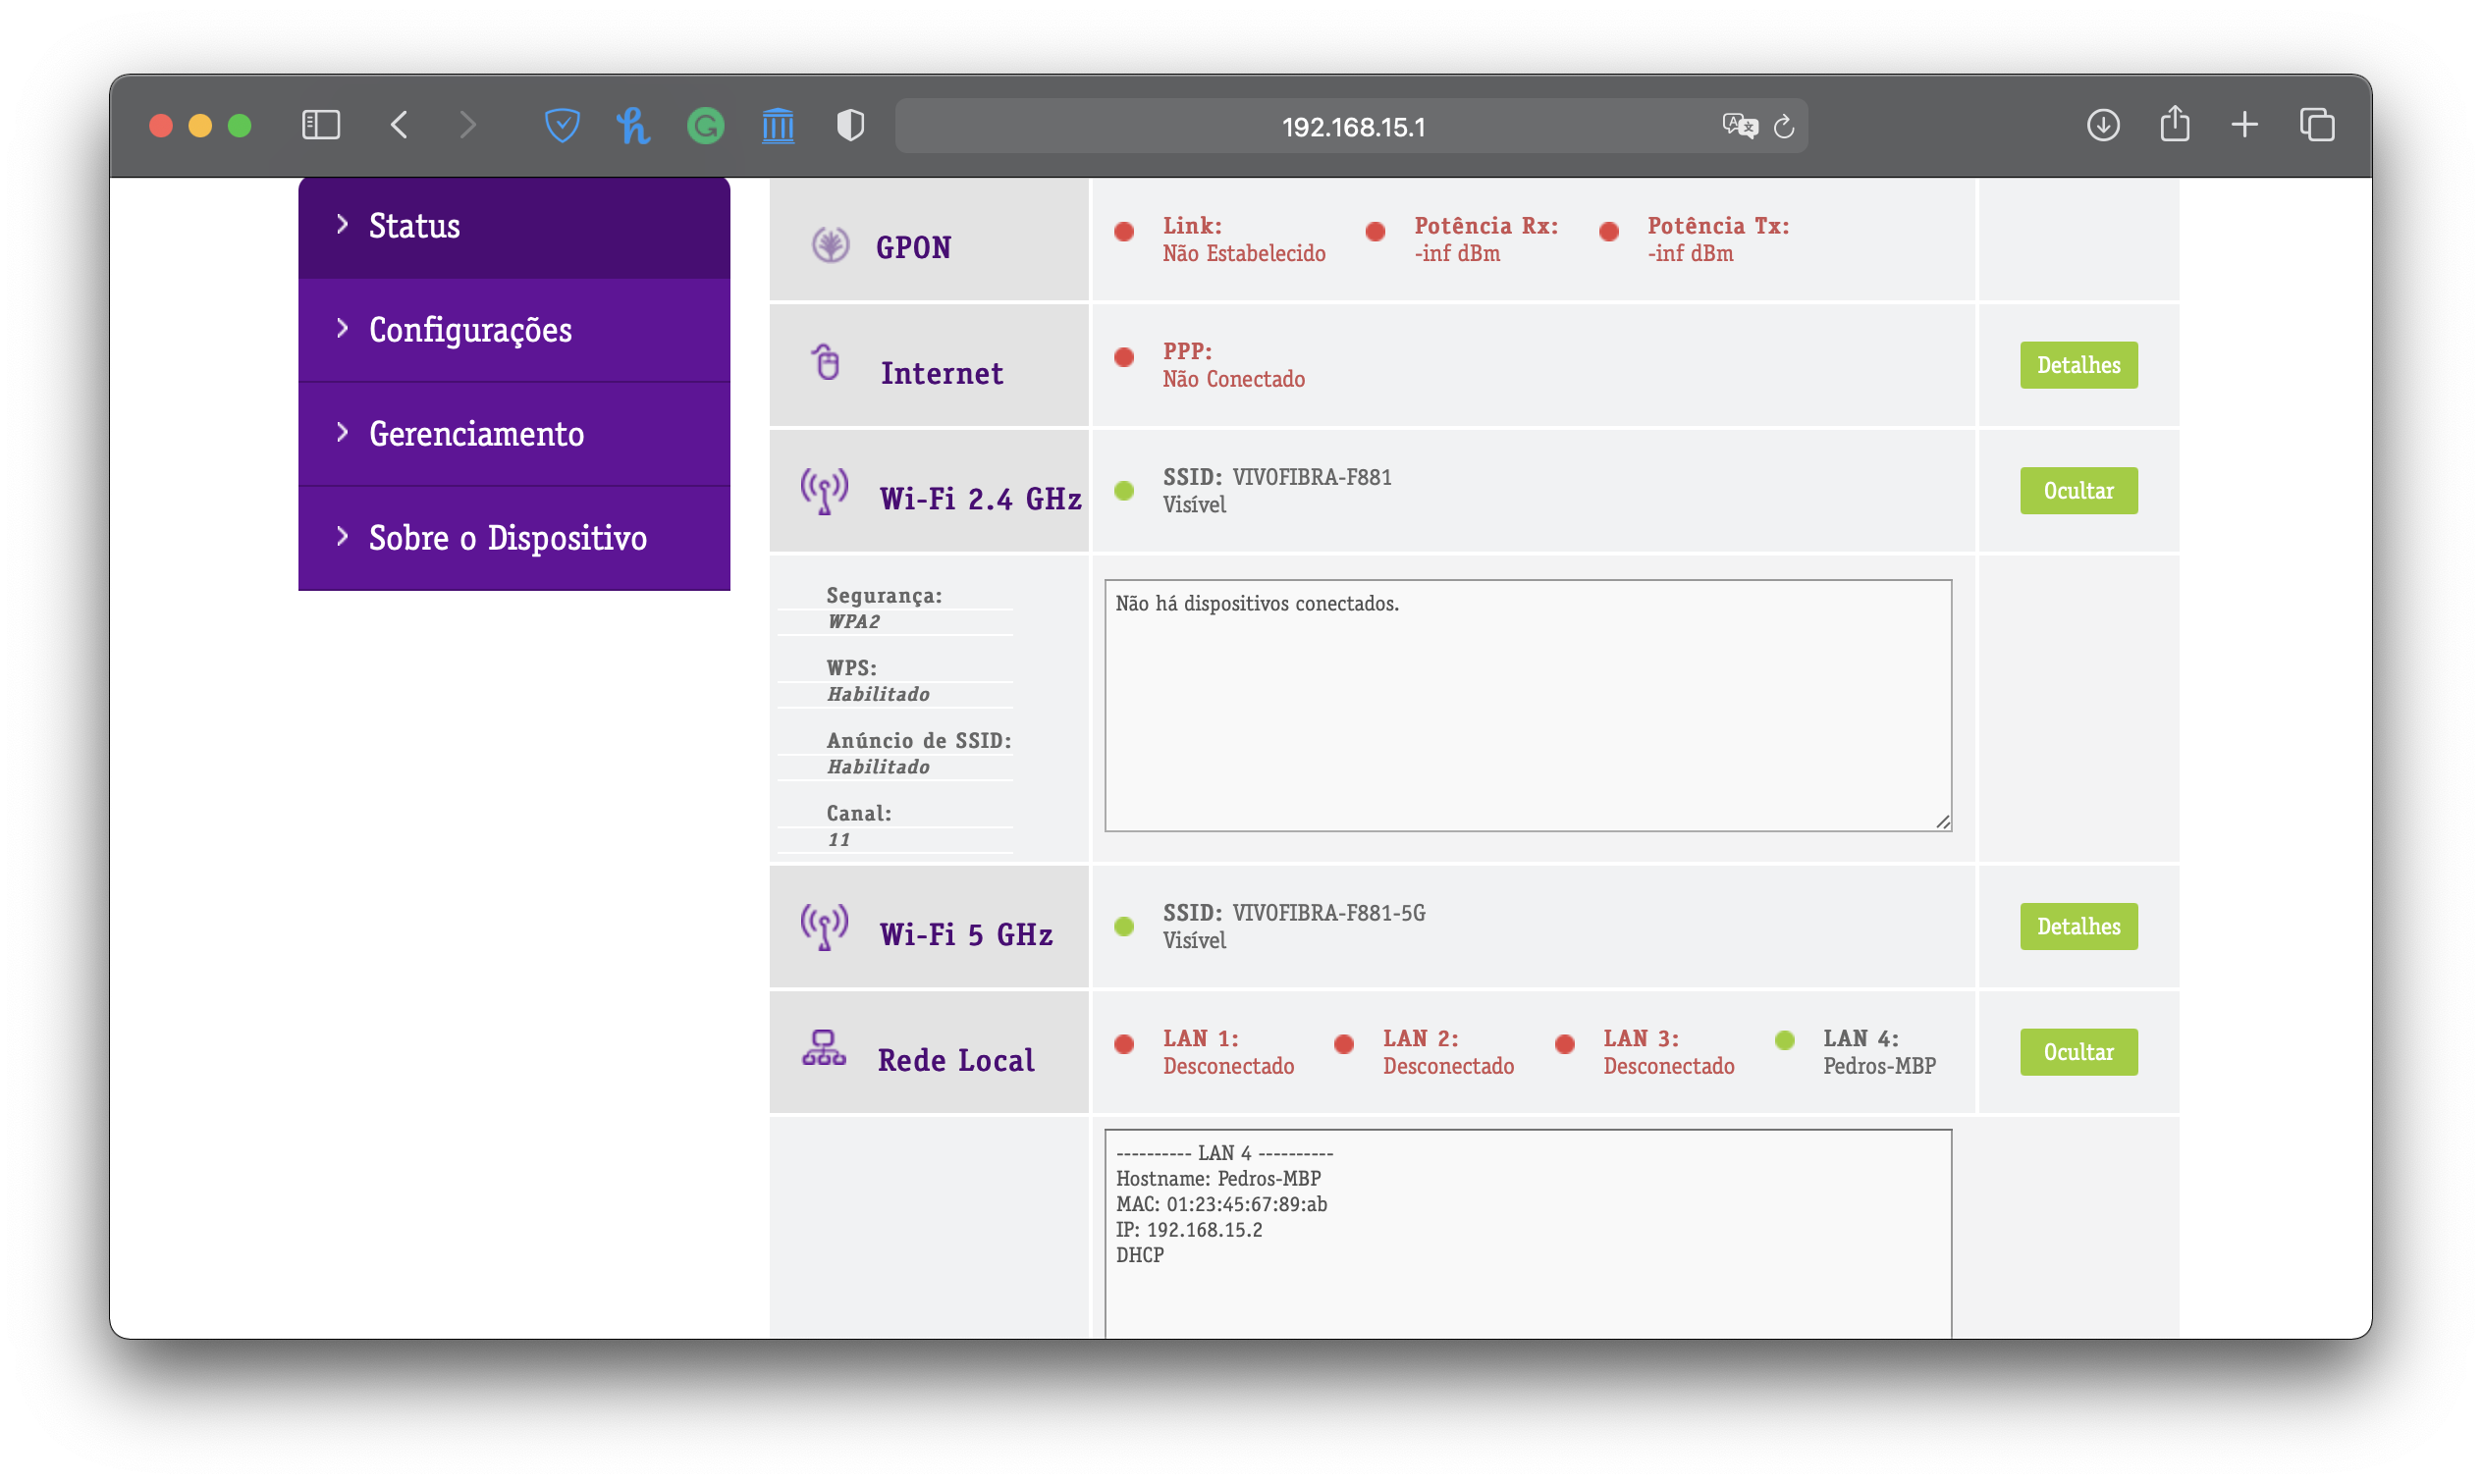
\includegraphics[width=\linewidth]{contents/cpes-and-research-data/anonymously-accessing-management-interfaces/main-page-cpe-http-management-interface.png}
    \caption{Main Page of the \gls{cpe} \gls{http} Management Interface}
    \label{figure:main_page_cpe_http_management_interface}
\end{figure}

The about page of the interface, Figure \ref{figure:about_page_cpe_http_management_interface}, shows the manufacturer, model, firmware version, hardware version, serial number, \gls{wan}-side \gls{mac} address, and \gls{lan}-side \gls{mac} address. If the device is fiber-compatible, it also shows the \gls{gpon} \gls{s/n}.

\begin{figure}[h]
    \centering
    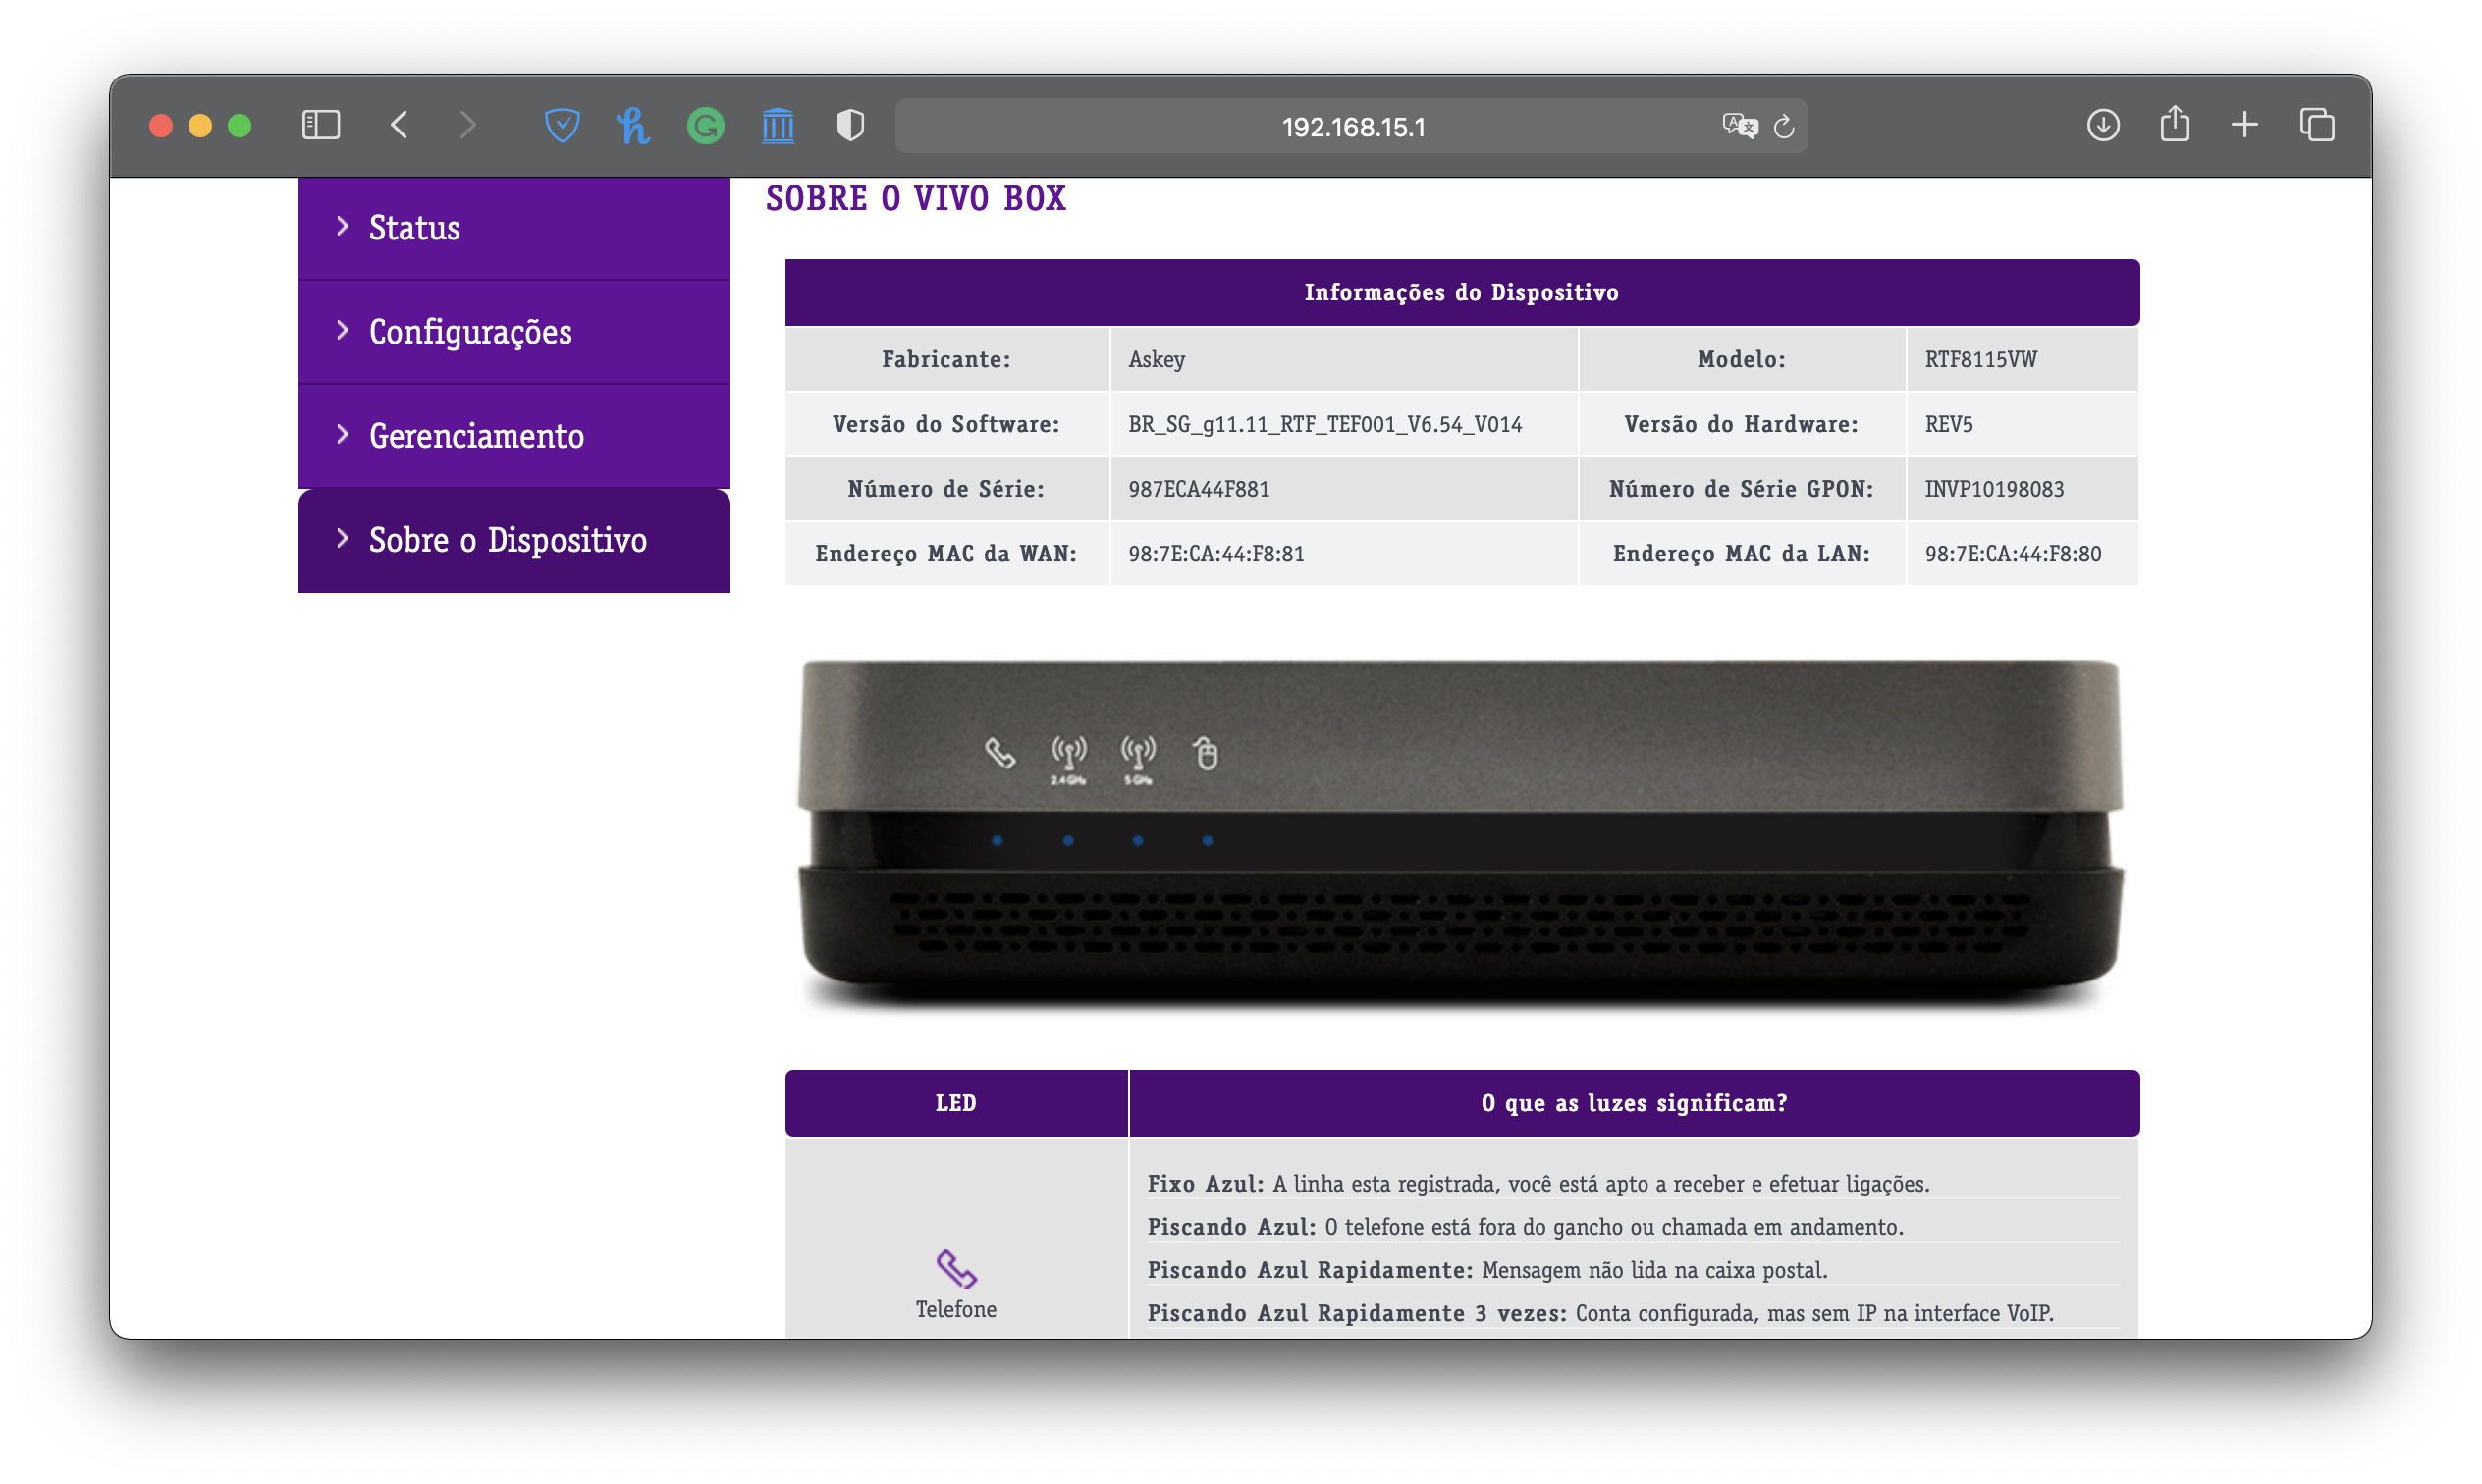
\includegraphics[width=\linewidth]{contents/cpes-and-research-data/anonymously-accessing-management-interfaces/about-page-cpe-http-management-interface.png}
    \caption{About Page of the \gls{cpe} \gls{http} Management Interface}
    \label{figure:about_page_cpe_http_management_interface}
\end{figure}

The \gls{ssh} and Telnet interfaces, even when manually enabled, don’t expose any data about the device without authenticating, immediately requesting credentials.

\FloatBarrier

\subsection{Configuration Export}

None of the \glspl{cpe} support exporting the configuration file on the standard \gls{http} Management Interface, even when signing in with the admin user. But a hidden interface is available in all devices and it allows the configuration file to be exported. To access this interface, you must navigate to \url{http://192.168.15.1/padrao} and log into the support user, using the admin’s password.

On \glspl{cpe} 2 to 7, you can navigate through the menu and export the configuration in the proper page with the support account. But \glspl{cpe} 0 and 1 don’t have the export page indexed in the menu, and you must access \url{http://192.168.15.1/saveconf.htm} manually, shown in Figure \ref{figure:cpe_saveconf}.

\begin{figure}[h]
    \centering
    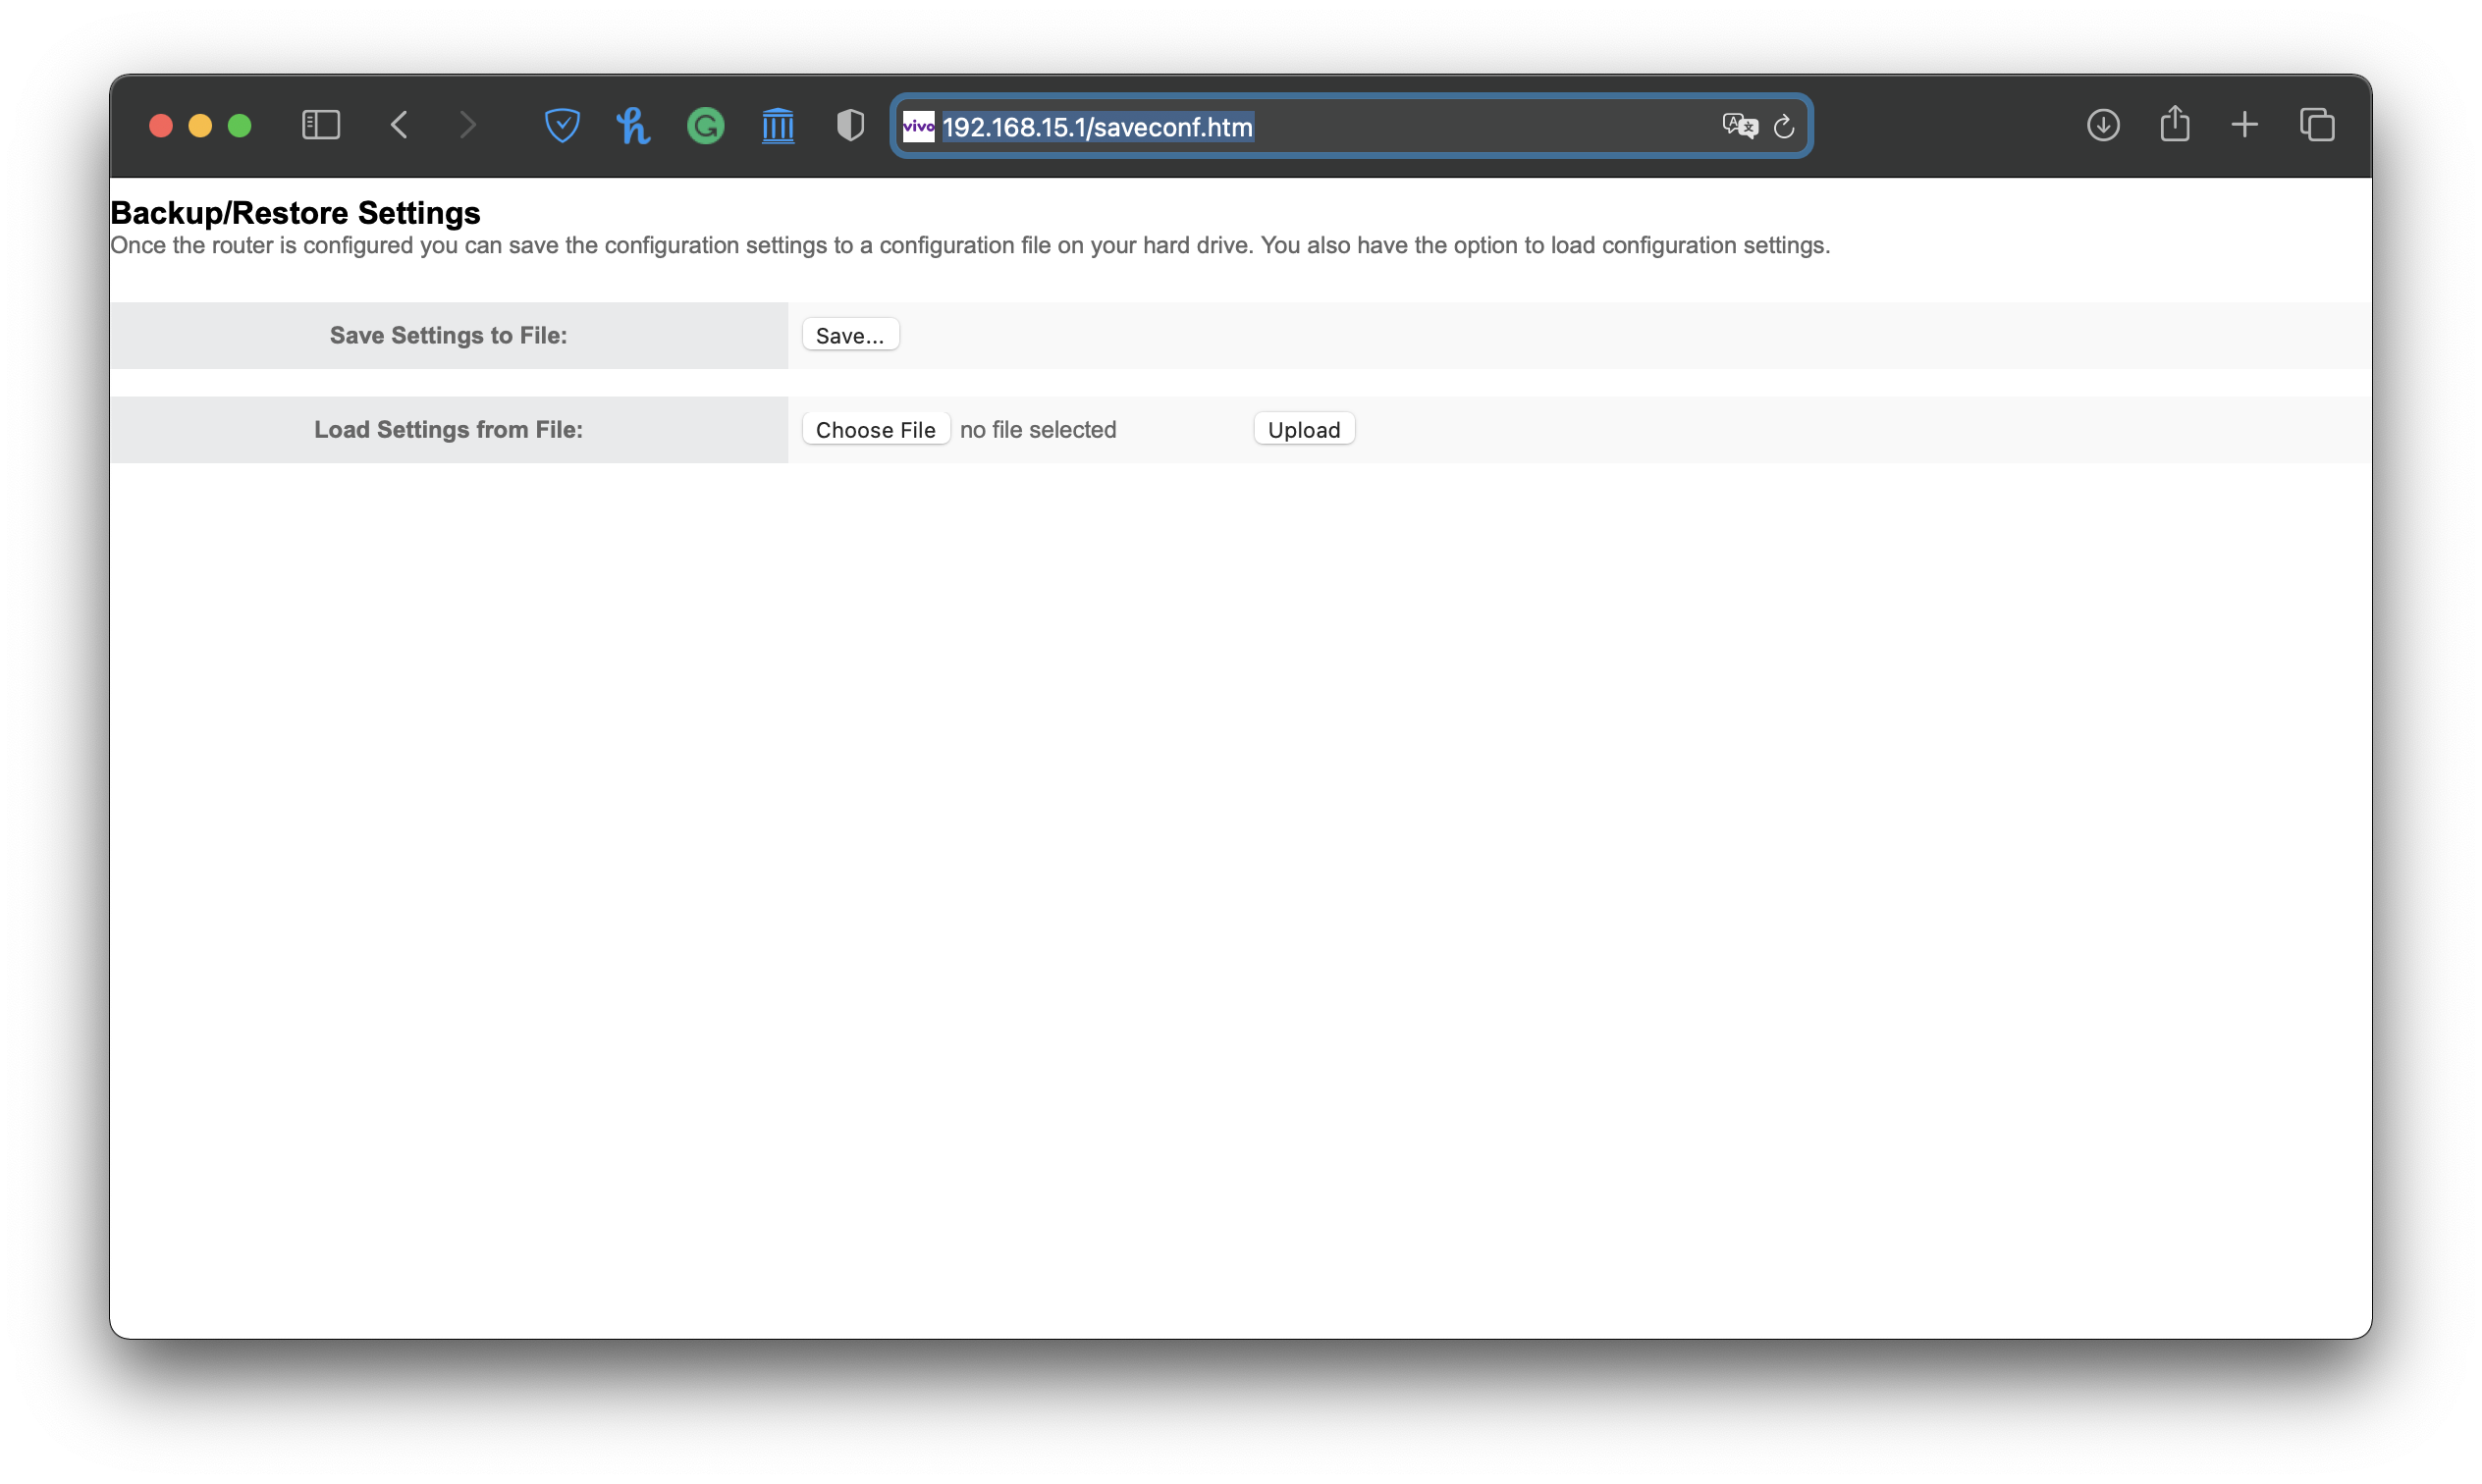
\includegraphics[width=\linewidth]{contents/cpes-and-research-data/configuration-export/cpe-saveconf.png}
    \caption{Unindexed \gls{cpe} Configuration Export Page}
    \label{figure:cpe_saveconf}
\end{figure}

\FloatBarrier

\subsection{EPROM Extraction}

The \glspl{cpe} don’t have any functionality intended to dump their \gls{eprom} via software. But it was discovered that by accessing \glspl{cpe} 4 to 7 via \gls{ssh} or Telnet, you are either able to read the memory area where the \gls{eprom} is mapped or read the \gls{mtd} partition with \gls{tftp} and dump it to a server. The command bellow can be executed on compatible \glspl{cpe} to have the first \gls{eprom} partition transfered to \url{192.168.15.2}, a \gls{tftp} server.

\begin{lstlisting}[language=Bash,numbers=none]
tftp -l /dev/mtd0 -p 192.168.15.2
\end{lstlisting}

To list all \gls{eprom} partitions, the \texttt{/proc/mtd} file can be read, as shown in Figure \ref{figure:cpe5_proc_mtd}.

\begin{figure}[h]
    \centering
    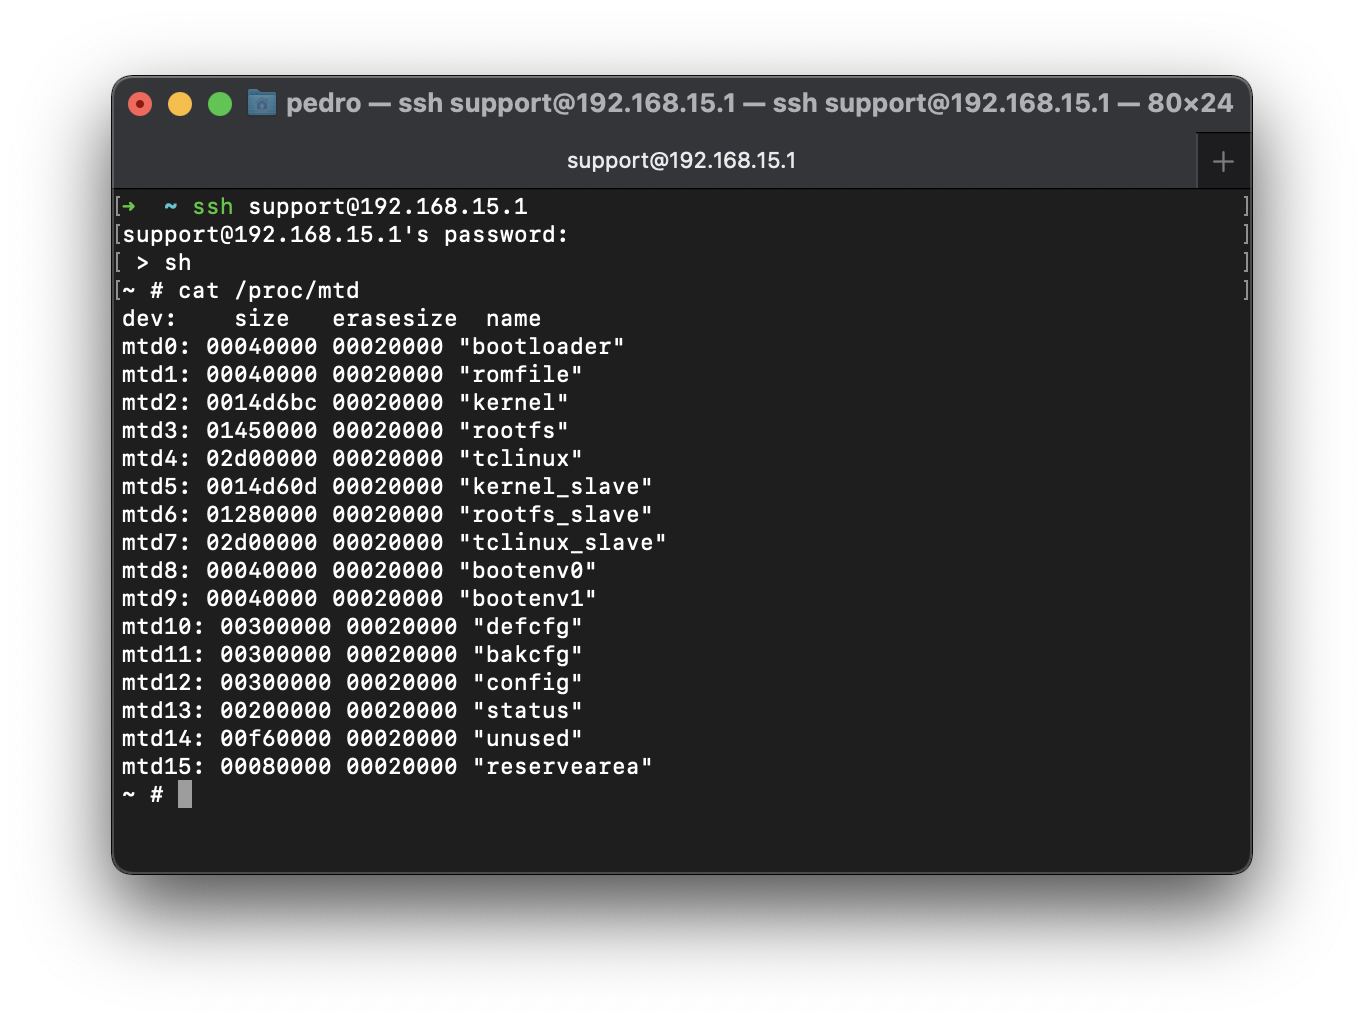
\includegraphics[width=\linewidth]{contents/cpes-and-research-data/eprom-extraction/cpe5-proc-mtd.png}
    \caption{File /proc/mtd of \gls{cpe} 5}
    \label{figure:cpe5_proc_mtd}
\end{figure}

Although it is possible to read the \gls{eprom} of \gls{cpe} 6 using the \gls{tftp} technique, the device’s shell sets a small time limit to processes executed from it, making it impossible to complete the transfer before the limit exceeds. To work around this problem, an \gls{eprom} programmer was directly attached to the \gls{cpe}’s \gls{eprom}, allowing a computer to dump its contents via the programmer.

On \glspl{cpe} 0 and 1, there is a command that shows the memory addresses where the \gls{eprom} is mapped and there is another command is capable of reading the content of an arbitrary memory address. Combining both commands, it is possible to extract the full \gls{eprom} content from a machine capable of accessing the \glspl{cpe} via Telnet. The scripts used are attached on Appendix \ref{appendix:cpe_eprom_ext}.

For \glspl{cpe} 2 and 3, the same technique of using an \gls{eprom} programmer had to be used. No command capable of dumping the \gls{eprom} via software was found.

\FloatBarrier

